

This chapter presents the empirical assessment performed to validate the test suite selection criteria described in Chapter \ref{chap:coverage} and the mutation analysis described in Chapter \ref{chap:mutation}. Each assessment is explained in a separate section. Each section starts with the research question(s) driving the assessment, describes the setup and results, and discuss those results and their validity. 

Section \ref{sec:experiment:allstates} presents the assessment of the all-states selection described in Section \ref{subsec:allstatesselection}; Section \ref{sec:experiment:dissimilarity} presents the assessment of the dissimilarity-based selection described in Section \ref{sec:coverage:dissimilaritycrit}; Section \ref{sec:experiment:beahviouralcoverage} assesses how classical feature model coverage criteria, like \textit{t}-wise, cover the behaviour of a product line using two state-of-the-art tools; and Section \ref{sec:experiment:usage} presents the assessment of the usage selection and prioritization criteria described in Section \ref{sec:coverage:usagecrit}. 

For mutation analysis, Section \ref{sec:experiment:fmmexec} presents the assessment of the mutants execution using \glspl{FMM} described in Section \ref{sec:FMM} in a product-based mutation analysis scenario. Finally, Section \ref{sec:experiment:mutequiv} presents the assessment of the mutant equivalence detection for products using automata language equivalence and simulation (described in Section \ref{sec:EMP}).



%%%%%%%%%%%%%%%%%%%%%%%%%%%%%%%%%%%%%%%%%%%
\section{All-states selection criteria}
%%%%%%%%%%%%%%%%%%%%%%%%%%%%%%%%%%%%%%%%%%%

\label{sec:experiment:allstates}

To assess the all-states selection algorithm described in Section \ref{subsec:allstatesselection}, we use coverage measures to answer to the following research question \cite{Devroey2014c}:
\begin{itemize}
\item \textbf{\textit{Coverage ability} } How does the coverage the selected test suite compare to the coverage of the randomly selected test suites?
\end{itemize}

%--------------------
\subsection{Setup}
%--------------------

Our evaluation has been performed on three case studies: the Soda vending machine (see section \ref{sec:casestudy:svm}), the Minepump (see section \ref{sec:casestudy:minepump}), and Claroline (see section \ref{sec:casestudy:claroline}). For each of them, we select random test suites and a test suite satisfying the all-states coverage criterion using Algorithm \ref{algo:allstatesheuristic}.

We select random test suites with the same number of test cases (\textit{random1}) as the ones selected by all-states algorithm (\textit{allstates}) to enable direct comparison of coverage. We also randomly select larger test suites (\textit{random2}) to figure out coverage gains. In total, for each model, we select one \textit{allstates} test suite and 100 \textit{random1} and \textit{random2} test suites. For the soda vending machine, the \textit{allstates} and \textit{random1} test suite contains 5 test cases, and the \textit{random2} test suite contains 20 test cases. The \textit{allstates} and \textit{random1} test suite of the Minepump contains 12 test cases and the \textit{random2} test suite contains 20 test cases. And for Claroline, the \textit{allstates} and \textit{random1} test suite contains 105 test case, and the \textit{random2} test suite contains 200 test cases. 

This assessment was performed on a Windows 7 machine with an Intel Core i3 (3.10GHz) processor and 4GB of memory. 

%--------------------
\subsection{Results}
%--------------------

\begin{figure}
	\centering
    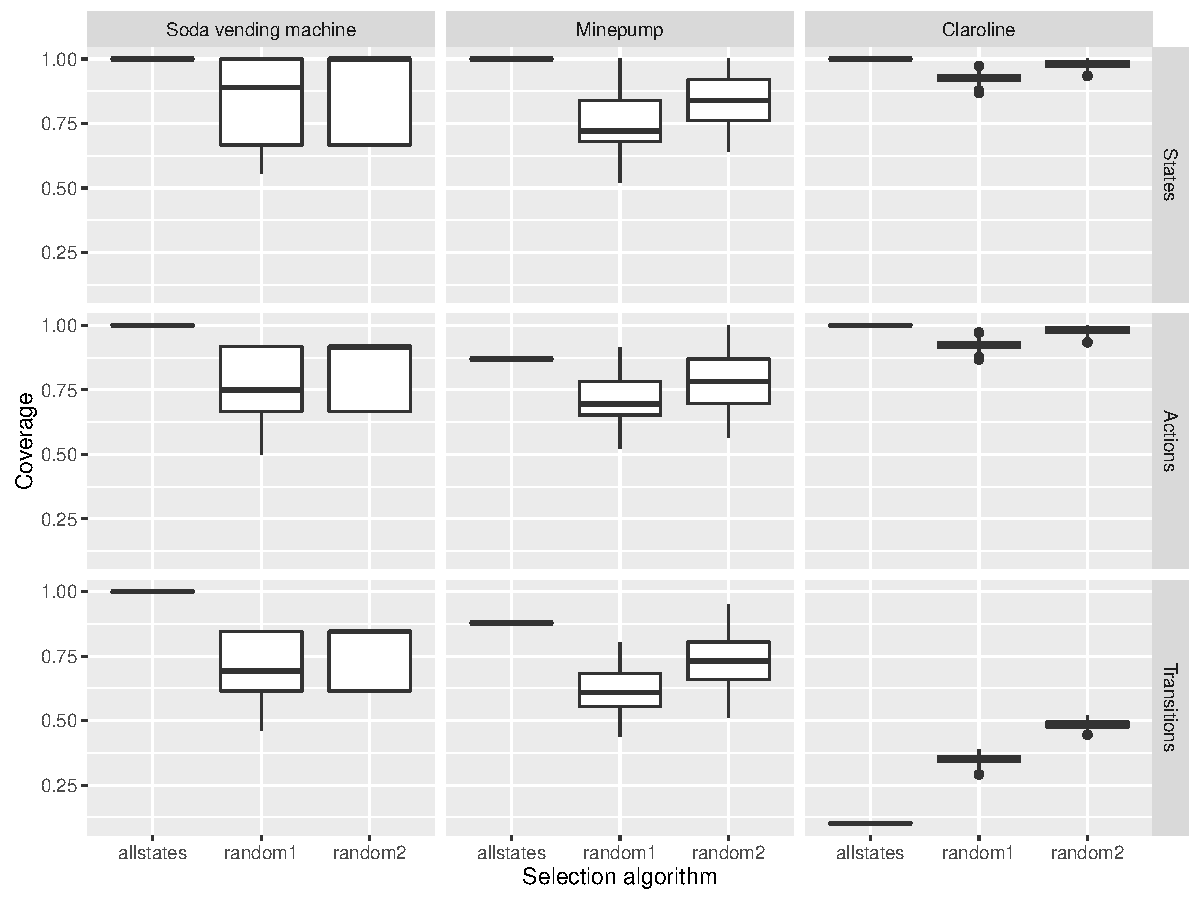
\includegraphics[width=\textwidth]{allstates-coverage}
	\caption{Structural coverages of the \textit{allstates}, \textit{random1}, and \textit{random2} test suites}
	\label{fig:allstatescoverage}
\end{figure}

Figure \ref{fig:allstatescoverage} presents the states, actions, and transitions coverage of the different test suites.  By construction, abstract test suites selected using our all-states algorithm (\textit{allstates} in Figure \ref{fig:allstatescoverage}) covers all the states for the three FTSs. On average, the random algorithm does not perform well to cover all the states of the different models.
On the contrary, the random algorithm performs better at covering transition on the largest model (Claroline): an average of 48.45\% for the 200 randomly selected test suites (\textit{random2}) against 10.17\% for the all-states selection algorithm.

%----------------------
\subsection{Discussion}
%----------------------

We investigated the difference between the \textit{allstates} and \textit{random(1,2)} transitions coverage for the Claroline model  and found that the all-states test suite contains only short test cases (2 actions). 
This is due to our heuristic. Since it prefers states that have a path to uncovered states, the initial state has the highest score in the Claroline model (because nearly all the states in the models have transitions coming from and going to the initial state, due to the web nature of the application). Changing the heuristic to avoid direct return to the initial state may improve the results for this kind of models (where each state is strongly connected to the initial state) but may increase the complexity of the algorithm and select inadequate abstract test cases for other kinds of models. 

These results are in line with the fact that all-states coverage criterion is poor to cover transitions in single systems \cite{Utting2007}, we assume that this is also the case for FTSs. Of courses an all-transitions algorithm would have given much better results (and all-states coverage). However our preliminary evaluation of such an algorithm resulted in huge scalability problems for the Claroline case study; after more than 3 days of selection and a text file describing the test suite of more 250 GB, our systems ran out  of memory (and also of hard drive space!).  Exhaustive computation of all-transitions for moderate size FTS is therefore not an option in most cases.    

Finally, we observe that the test suite selected to cover all-states in the Claroline FTS also covers all the actions. This is due to the nature of the model, since each state represents a page and each action represents a link followed from a page (\ie a state in the FTS) to another page (\ie another state), there are as many actions as there are states. Each action is thus covered. This is not always the case, \eg the soda vending machine in Figure \ref{fig:allstatescoverage}.

%--------------------------------
\subsection{Threats to validity}
%--------------------------------

\paragraph{Internal validity:}
%----------------------------

The all-states selection algorithm has been simplified to reduce the number of SAT calls which are very costly. This simplification gives good results on our largest model (Claroline) due to the few constraints on the FTS. On other models with more constraints on the different transitions, this simplification may give poor results since it can potentially select a lot of invalid test cases. We intend to compare the actual implementation which uses a SAT solver with binary decision diagrams (BDDs) which have performed better when processing FTSs \cite{Classen2011}.

The random selection of a test suite does not check whether there are duplicates abstract test cases or not. Since the size of the test suites considered for \textit{random2} test suites is larger than the size of the all-states covering test suite, this thread is limited. To avoid this, one may implement a filter to check that newly selected test suites are not duplicated.

\paragraph{Construct validity:}
%----------------------------

The Claroline FTS and its FM contain few constraints ending in a SPL with lots of products. We believe this is a typical characteristic of web applications which are a particular class of system. This has influenced the implementation of the random algorithm in order to minimize the number of SAT calls (which are costly in CPU time). It has also influenced the heuristic during the selection of the test suite covering all-states and gives very short test cases in regard to the size of the system. We plan to apply our algorithms on large industrial systems with more constrained FM and FTSs in order to validate our conclusions.

\paragraph{External validity:}
%----------------------------

To avoid too many SAT calls, we verify that an abstract test case is executable \textit{a posteriori} by calling the SAT solver once with the conjunction of the FM (represented as a boolean formula) and the feature expression of the transitions of the test case. We repeat the building of an abstract test case while it is not executable. Since the largest FTS model we considered does not have a lot of behaviours exclusive to subsets of the product line, this implementation of the random algorithm works fast. This may be not the case for other models with a lot of constrained behaviour.

As discussed by Inozemtseva et al. \cite{Inozemtseva2014}, a test suite with a good coverage does not guarantee the effectiveness of this test suite. However, in a first attempt to compare our selection algorithms, coverage seems to be a reasonable metric.


%%%%%%%%%%%%%%%%%%%%%%%%%%%%%%%%%%%%%%%%%%%
\section{Dissimilarity selection criteria}
%%%%%%%%%%%%%%%%%%%%%%%%%%%%%%%%%%%%%%%%%%%

\label{sec:experiment:dissimilarity}

We report hereafter on our evaluation of dissimilarity driven test suite selection \cite{Devroey2016}. In order to compare the different dissimilarity selections, we define the following research questions:
\begin{itemize}
\item \textbf{\textit{Dissimilarity relevance} (RQ.1) } How does the similarity-driven search based approach compare to all-actions and random test selection with respect to fault finding and product coverage?
\item \textbf{\textit{Distance impact} (RQ.2) } How does the choice of a given distance influences the results?
\end{itemize}


%--------------------
\subsection{Setup}
%--------------------

\label{sec:assessment:dissimilarity:setup}

We consider 4 models from different sources with different sizes as input to different test case selection processes. The four model are: the Soda vending machine (see section \ref{sec:casestudy:svm}), the Minepump (see section \ref{sec:casestudy:minepump}), the card payment terminal (see section \ref{sec:casestudy:cpterminal}), and Claroline (see section \ref{sec:casestudy:claroline}). In order to avoid bias using random selection, we run the evaluation 6 times for each model and each configuration of the algorithm (6 configurations overall) presented in this section.

\paragraph{Test suites selection:}
%---------------------------------

\begin{table}
	\centering
	\caption{Number of test cases and selection time of the all-actions test suites}
	\begin{small}
	\begin{tabular}{lrrrr}
		\hline
		\textbf{Model}	& \multicolumn{2}{c}{\textbf{Time ($d_{allactions}$)}} 	& \multicolumn{2}{c}{\textbf{Test cases ($k_{allactions}$)}}\\
						& $\overline{time}$ & $\sigma$		& $\overline{count}$	& $\sigma$	\\
		\hline 
		S. V. Mach.		& 1.03 sec. & 0.093	& 3.86	& 0.35	\\
		Minepump			& 1.18 sec. & 0.189	& 11.14	& 0.99	\\
		C. P. Term.		& 1.24 sec.	& 0.263	& 5.0	& 0.76	\\
		Claroline		& 3.42 sec.	& 1.814	& 52.86	& 2.95	\\
		\hline
	\end{tabular}
	\end{small}
	\label{tab:allactions:exec}
\end{table} 

For each model, we select a test suite which satisfies the \emph{all-actions} coverage criteria (\ie when executing all the test cases, all the actions of the FTS are executed at least once). We measure the selection time ($d_{allactions}$) and the number of test cases ($k_{allactions}$) and report in Table \ref{tab:allactions:exec}. 
%
The \emph{number of test cases} and the \emph{selection time} are used as input for the dissimilar test suite selections. To assess time impact ($d$  in Algorithm \ref{algo:diss}) on the results, we consider the following values: $1 \times d_{allactions}$, $2 \times d_{allactions}$, $10 \times d_{allactions}$, and $100 \times d_{allactions}$ to parametrize the time during which the evolutionary algorithm runs. 
%
We configure the algorithm using different \emph{distances} to compute the fitness function: the Jaccard index for product dissimilarity; and the Hamming distance, Jaccard index, dice and anti-dice, and Levenshtein distances for actions dissimilarity. We combine product dissimilarity and actions dissimilarity using the multiplication and average operator ($\otimes$), and also consider action dissimilarity alone. For each configuration, we run the algorithm  using local and global distances for the sort.
%
For each model, A \emph{random} suite of $k_{allactions}$ test cases is also selected (see Algorithm \ref{algo:random}). In total, we selected 122 test suites for each model.


\paragraph{Fault injection and test suites execution:}
%------------------------------------------------------

\begin{table}
	\centering
	\caption{Number of faulty states, transitions, and actions seeded in the models}
	\begin{small}
	\begin{tabular}{lrrrrrr}
		\hline
		\textbf{Model}	& \multicolumn{2}{c}{\textbf{Faulty States}}	& \multicolumn{2}{c}{\textbf{Faulty Transitions}} & \multicolumn{2}{c}{\textbf{Faulty Actions}} \\
						& \textit{$\overline{faults}$} & \textit{$\sigma$}	& \textit{$\overline{faults}$} & \textit{$\sigma$}	& \textit{$\overline{faults}$} & \textit{$\sigma$}\\
		\hline 
		S. V. Mach.		& 4.6	& 0.8	& 5.9	& 1.0	& 5.7	& 1.0	\\
		Minepump			& 12.4	& 1.4	& 19.3	& 1.7	& 9.6	& 1.5	\\
		C. P. Term.		& 5.3	& 0.9	& 7.9	& 1.1	& 6.8	& 1.1	\\
		Claroline		& 52.1	& 2.9	& 896.8	& 13.3	& 32.3	& 2.9	\\
		\hline
	\end{tabular}
	\end{small}
	\label{tab:avg:faults}
\end{table}

Fault seeding is a popular technique to assess and compare test suites coverage \cite{Andrews2005,Andrews2006,Mathur2008}. The idea is to inject faults in SUT and measure the number of faults detected by the test suite. 
%In a SPL context, fault injection (using mutation testing) has been applied to feature models by Henard et al. \cite{Henard2013b}. 
%We did not consider fault injection in the FM, in place 
In this evaluation, we choose to artificially inject faults into the FTS by tagging state, transitions and actions as faulty. We randomly select states, transitions, and actions to assume them as faulty (\ie containing a fault), if a state/transition/action is selected more than once, it is only counted as 1 during the fault detection. We then execute the test suites on the FTS and consider that a fault is revealed as soon as the faulty states is reached, the faulty transitions are fired, and the faulty actions are executed.
Using information coming from previous versions of the system (\ie from a bug tracker), this would allow one to tag elements of the model that are more likely to contain faults.
In our case, we do not have access to such information and use a random selection with an upper bound of 66\% of faults of the states, actions, and transitions of the FTS. This gives a measure is close to states, actions, and transitions coverage but still allows to finely compare the different approaches. Table \ref{tab:avg:faults} presents the average number of faults seeded in the different models during the evaluation.

%--------------------
\subsection{Results}
%--------------------

\begin{figure}
	\centering
	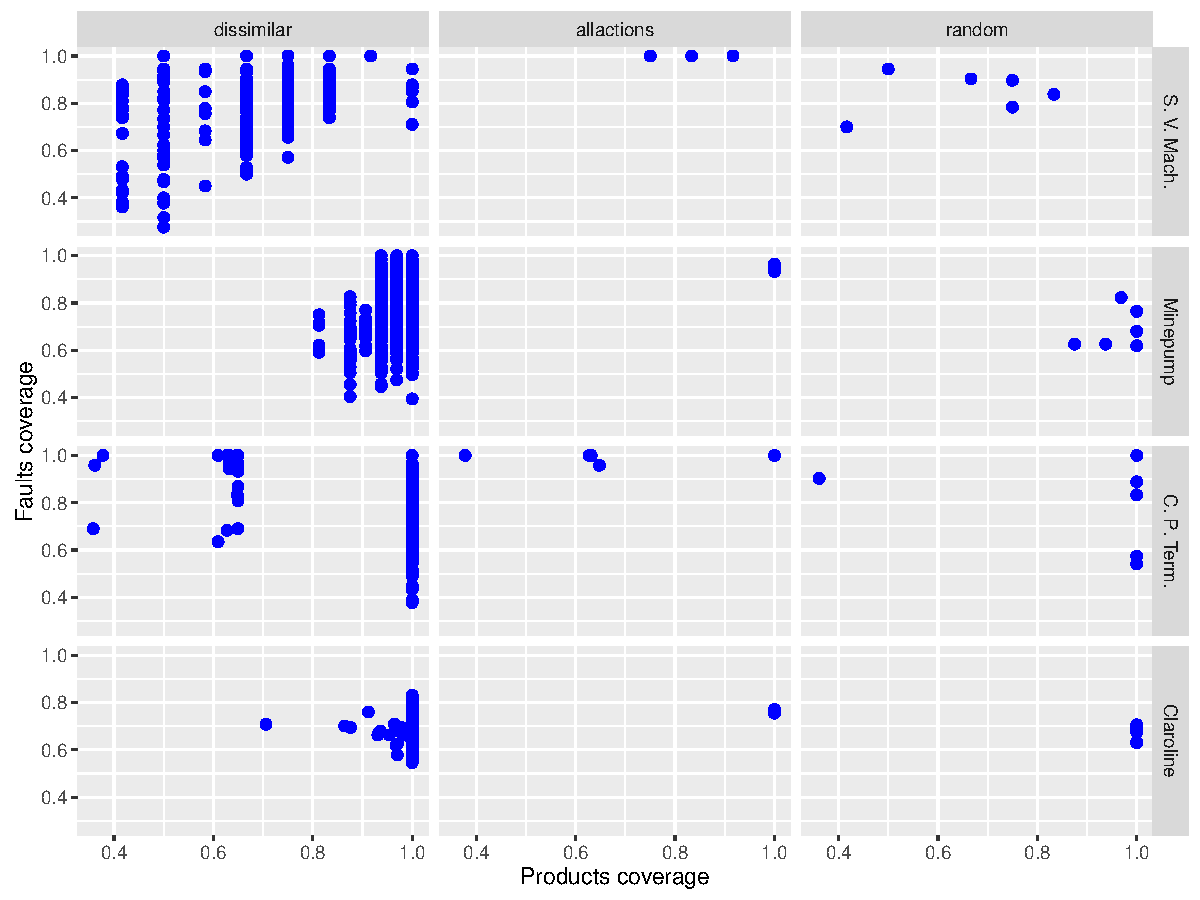
\includegraphics[width=0.98\textwidth]{diss-coverages}
	\caption{Faults coverage of the all-actions, random, and dissimilar test suites}
	\label{fig:assessment:faultscoverage}
\end{figure}

Figure \ref{fig:assessment:faultscoverage} presents the coverage distribution of the different test suites selected using dissimilarity, all-actions coverage, and random algorithm. The x-axis is the percentage of products covered by the test suite: for a suite $s$ and a feature model $d$, it corresponds to $\frac{\#prod(d, s)}{\# [\![d]\!]}$. The y-axis is the percentage of faults (states, transitions, or actions) discovered when executing the test suite.

To characterize the test suites (\ie, the solution space of our bi-objective selection), we compute a \emph{reference front}, by taking the Pareto front of \emph{all} the points in Figure \ref{fig:assessment:faultscoverage}. This reference front contains all the sets of test cases maximising the fault and products coverages (\ie, the best solutions). We give hereafter for each model a podium with the 3 (or more if they have the same frequency) optimal configurations of the dissimilarity-based selection providing solutions that are on the reference front:
\begin{itemize}
\item \textbf{Soda vending machine} (47 optimal solutions)
	\begin{itemize}
	\item Hamming avg., global, $t=10$ ($freq. = 0.056$)
	\item Hamming avg., global, $t=1$ ($freq. = 0.056$)
	\item Hamming avg., global, $t=2$ ($freq. = 0.056$)
	\item Hamming avg., global, $t=100$ ($freq. = 0.056$)
	\end{itemize}
\item \textbf{Minepump} (6 optimal solutions)
	\begin{itemize}
	\item Jaccard sing., global, $t=2$ ($freq. = 0.222$)
	\item Jaccard avg., global, $t=10$ ($freq. = 0.222$)
	\item Antidice sing., global, $t=1$ ($freq. = 0.222$)
	\end{itemize}
\item \textbf{Card payment terminal} (64 optimal solutions)
	\begin{itemize}
	\item Levenshtein sing., global, $t=2$ ($freq. = 0.029$)
	\item Antidice sing., global, $t=10$ ($freq. = 0.029$)
	\item Levenshtein sing., global, $t=2$ ($freq. = 0.029$)
	\item Antidice mul., global, $t=2$ ($freq. = 0.029$)
	\item Antidice avg., global, $t=2$ ($freq. = 0.029$)
	\end{itemize}
\item \textbf{Claroline} (1 optimal solution)
	\begin{itemize}
	\item Hamming sing., global, $t=100$ ($freq. = 1.0$)
	\end{itemize}
\end{itemize}


\begin{table}
	\centering
	\caption{Hypervolumes values for the Claroline case-study}
	

%\begin{tabular}{l r c c c c c c  c c c  c c c  c c c }
%\hline
%% Titles
%\multicolumn{2}{r}{ } & \multicolumn{15}{c}{\textbf{Actions dissimilarity distance}} \\
%% Selection criteria
%\multicolumn{2}{r}{ } & \multicolumn{3}{c}{\textbf{Hamming}} & \multicolumn{3}{c}{\textbf{Jaccard}} & \multicolumn{3}{c}{\textbf{Dice}} & \multicolumn{3}{c}{\textbf{Antidice}} &  \multicolumn{3}{c}{\textbf{Levenshtein}}\\
%% Mul and Avg
%& \textit{t} & \textit{Avg.} & \textit{Mul.} & \textit{Sing.} & \textit{Avg.} & \textit{Mul.} & \textit{Sing.} & \textit{Avg.} & \textit{Mul.} & \textit{Sing.} & \textit{Avg.} & \textit{Mul.} &  \textit{Sing.} & \textit{Avg.} & \textit{Mul.} & \textit{Sing.} \\ 
%\hline
%% Values
% & \textit{1} & 0.688 & 0.662 & 0.690 & 0.673 & 0.705 & 0.690 & 0.693 & 0.709 & 0.690 & 0.711 & 0.692 & 0.668 & 0.691 & 0.722 & 0.691 \\
%\textbf{Loc.} & \textit{2} & 0.674 & 0.699 & 0.705 & 0.679 & 0.673 & 0.684 & 0.667 & 0.689 & 0.670 & 0.688 & 0.690 & 0.659 & 0.666 & 0.662 & 0.677\\
%\textbf{sort} & \textit{10} & 0.702 & 0.681 & 0.661 & 0.721 & 0.685 & 0.700 & 0.720 & 0.669 & 0.679 & 0.667 & 0.674 & 0.651 & 0.691 & 0.681 & 0.696 \\
% & \textit{100} & 0.667 & 0.693 & 0.672 & 0.672 & 0.720 & 0.713 & 0.691 & 0.703 & 0.678 & 0.696 & 0.685 & 0.655 & 0.655 & 0.678 & 0.687 \\
% & \textit{1} & 0.736 & 0.710 & 0.724 & 0.694 & 0.697 & 0.727 & 0.695 & 0.683 & 0.710 & 0.666 & 0.672 & 0.699 & 0.684 & 0.693 & 0.717 \\
%\textbf{Glob.} & \textit{2} & 0.711 & 0.708 & 0.755 & 0.722 & 0.718 & 0.715 & 0.723 & 0.670 & 0.729 & 0.677 & 0.705 & 0.728 & 0.708 & 0.687 & 0.733 \\
%\textbf{sort} & \textit{10} & 0.740 & 0.733 & 0.804 & 0.723 & 0.696 & 0.730 & 0.690 & 0.683 & 0.738 & 0.701 & 0.692 & 0.746 & 0.701 & 0.714 & 0.771 \\
% & \textit{100} & 0.794 & 0.800 & 0.831 & 0.747 & 0.729 & 0.756 & 0.750 & 0.714 & 0.755 & 0.747 & 0.740 & 0.758 & 0.747 & 0.730 & 0.781 \\	
%\hline
%\multicolumn{2}{l}{\textbf{All-act. crit.}}	& \multicolumn{15}{l}{0.771} \\
%\multicolumn{2}{l}{\textbf{Rand. crit.}}	& \multicolumn{15}{l}{0.706}  \\
%\end{tabular}


\begin{small}
\begin{tabularx}{0.98\textwidth}{X r  c c c  c c c  c c c}
%\begin{tabular}{l r  c c c  c c c  c c c}
\hline
% Selection criteria
\multicolumn{2}{r}{} & \multicolumn{3}{c}{\textbf{Hamming}} & \multicolumn{3}{c}{\textbf{Jaccard}} & \multicolumn{3}{c}{\textbf{Dice}} \\
% Mul and Avg
& \textit{t} & \textit{Avg.} & \textit{Mul.} & \textit{Sing.} & \textit{Avg.} & \textit{Mul.} & \textit{Sing.} & \textit{Avg.} & \textit{Mul.} & \textit{Sing.} \\ 
\hline
% Values
 				& \textit{1} & 0.688 & 0.662 & 0.690 & 0.673 & 0.705 & 0.690 & 0.693 & 0.709 & 0.690 \\
\textbf{Loc.}	& \textit{2} & 0.674 & 0.699 & 0.705 & 0.679 & 0.673 & 0.684 & 0.667 & 0.689 & 0.670 \\
\textbf{sort}	& \textit{10} & 0.702 & 0.681 & 0.661 & 0.721 & 0.685 & 0.700 & 0.720 & 0.669 & 0.679 \\
				& \textit{100} & 0.667 & 0.693 & 0.672 & 0.672 & 0.720 & 0.713 & 0.691 & 0.703 & 0.678 \\
 				& \textit{1} & 0.736 & 0.710 & 0.724 & 0.694 & 0.697 & 0.727 & 0.695 & 0.683 & 0.710 \\
\textbf{Glob.}	& \textit{2} & 0.711 & 0.708 & 0.755 & 0.722 & 0.718 & 0.715 & 0.723 & 0.670 & 0.729 \\
\textbf{sort}	& \textit{10} & 0.740 & 0.733 & 0.804 & 0.723 & 0.696 & 0.730 & 0.690 & 0.683 & 0.738 \\
				& \textit{100} & 0.794 & 0.800 & 0.831 & 0.747 & 0.729 & 0.756 & 0.750 & 0.714 & 0.755 \\
\hline
\end{tabularx}
%\end{tabular}

\begin{tabular}{l r  c c c  c c c}
 % Selection criteria
\multicolumn{2}{r}{ } & \multicolumn{3}{c}{\textbf{Antidice}} &  \multicolumn{3}{c}{\textbf{Levenshtein}}  \\
% Mul and Avg
& \textit{t} & \textit{Avg.} & \textit{Mul.} & \textit{Sing.} & \textit{Avg.} & \textit{Mul.} & \textit{Sing.}\\	
\hline
% Values
              & \textit{1} 	& 0.711 & 0.692 & 0.668 & 0.691 & 0.722 & 0.691 \\
\textbf{Loc.} & \textit{2} 	& 0.688 & 0.690 & 0.659 & 0.666 & 0.662 & 0.677 \\
\textbf{sort} & \textit{10} 	& 0.667 & 0.674 & 0.651 & 0.691 & 0.681 & 0.696 \\
              & \textit{100}	& 0.696 & 0.685 & 0.655 & 0.655 & 0.678 & 0.687 \\
              & \textit{1} 	& 0.666 & 0.672 & 0.699 & 0.684 & 0.693 & 0.717 \\
\textbf{Glob.}& \textit{2} 	& 0.677 & 0.705 & 0.728 & 0.708 & 0.687 & 0.733 \\
\textbf{sort} & \textit{10} 	& 0.701 & 0.692 & 0.746 & 0.701 & 0.714 & 0.771 \\
              & \textit{100}	&  0.747 & 0.740 & 0.758 & 0.747 & 0.730 & 0.781  \\
\hline
\end{tabular}

\begin{tabular}{c c}
\textbf{All-action}	& \textbf{Random}	\\
\hline
 0.771 & 0.706 \\
\hline
\end{tabular}

\end{small}

	\label{tab:claroline:hypervolumes}
\end{table}

Finally, Table \ref{tab:claroline:hypervolumes} presents hypervolume for the Claroline model for the different test suites. The hypervolume corresponds, for a test suite $s$, to the volume of the solution space dominated by $s$ \cite{Brockhoff2008,Henard2015}. A high value of hypervolume correspond to a set of test cases with a better fault and product coverage.
Rows and columns show the parameters values used for dissimilarity-based selection: the top rows indicate the actions dissimilarity distance ($diss_a$) and the operator ($\otimes$) used to combine it with the product distance ($diss_p$) or if the actions dissimilarity distance is used alone, \ie  in a single-objective configuration of the algorithm (denoted by \textit{Sing.} in the table); the leftmost columns indicate which sorting method is used (global or local) and the time considered for the algorithm ($1 \times d_{allactions}$, $2 \times d_{allactions}$, $10 \times d_{allactions}$, or $100 \times d_{allactions}$). 

The raw results for the 6 executions of the different test case selection algorithms and their fault finding evaluation may be downloaded at \url{http://projects.info.unamur.be/vibes}


%----------------------
\subsection{Discussion}
%----------------------

\paragraph{Dissimilarity relevance:} 
%-----------------------------------

Regarding \emph{RQ.1}, dissimilarity-based approaches are always able to obtain the optimal results in terms of fault finding ability and coverage.  On the three small models, these results are sometimes matched by the all-actions and random approaches (Figure \ref{fig:assessment:faultscoverage}).  However, the latter appear less frequently: neither random  nor all-actions are on the podium of optimal solutions in terms of frequency. Additionally on the Claroline case study, the only optimal solution found is a search-based one. We therefore confirm the good results of similarity-driven testing for single product testing \cite{Mondal2015} and product selection at the feature model level \cite{Henard2014a} for behavioural test case selection in an SPL context. 

The most important finding is that being fully bi-objective is not necessarily an advantage: on the 13 approaches present in the frequency podiums, only 6 are bi-objective. Additionally, a single objective approach dominates alone the Claroline case. This may be due to the nature of the case study, which is not heavily constrained: it is easy to obtain by chance dissimilar products. All-actions performance may benefit of this situation as well. Time may  be involved in the explanation: for a given amount of time, a bi-objective configuration will necessarily iterate less than a single-objective one.  

When bi-objective is optimal, the average (\textit{Avg.}) composition operator gives the best results as only one \textit{Mul.} approach appears on our podiums. Time given to the search-based algorithm has an (expected)  influence on the quality of the results.  This is apparent on the Claroline case where the best hypervolumes  are obtained by approaches that are given $t=100$.       

\paragraph{Distance impact:}
%---------------------------

If we consider all the podiums, Hamming and Jaccard-based distances (Dice, Antidice, Jaccard)  clearly win over Levenshtein.  This may seem surprising since Levenshtein  is the only one that is sequence-based taking into account the order of the actions.  Levenshtein is more computationally expensive than Hamming and Jaccard-based distances, implying less iterations of the algorithm for a given amount of time.  When employed alone (single-objective) on actions, it appears to be the second most performing distance on the Claroline case.       


%--------------------------------
\subsection{Threats to validity} 
%--------------------------------

%\paragraph{Construct validity:}
%---------------------------

To keep the comparison fair between the different test suite selection algorithms, we use the same number of test cases and duration time of the all-actions test suite selection to parametrize random and dissimilar test suites selections. As the dissimilar test suite selection is based on a (1+1) evolutionary algorithm \cite{Droste2002}, it is very sensitive to the maximal execution time ($d$). The all-actions test suite selection may be very fast (for the soda vending machine for instance). In order to assess the time influence in the quality of selection for the evolutionary approach, we chose to repeat the test case selection with different $d$ values.

We chose to use a (1+1) evolutionary algorithm \cite{Droste2002} to maximize the dissimilarity of the selected test suite. This algorithm is simple and to parametrize, and it showed good results to select products to test \cite{Henard2014a}. Many other algorithms, like adaptive random testing \cite{Chen2010}, used to select dissimilar test cases exist \cite{Hemmati2013}. A comparison between those different algorithms is left for future work.

The complete process described in Section \ref{sec:assessment:dissimilarity:setup} has been repeated 6 times for each model on a Ubuntu Linux machine (Linux version 3.13.0-65-generic, Ubuntu 4.8.2-19ubuntu1) with an Intel Core i3 (3.10GHz) processor and 4GB of memory. The complete experiment took approximately 4 days.

%\paragraph{External validity:}
%%---------------------------
%
%We cannot guarantee that our models are representative of real behavioural models. The soda vending machine, Minepump, and card payment terminal models are small with few states and transitions. The Claroline model is a larger model reverse engineered from a running web application, this gave us a model with a very flexible navigation (\ie a large number of transitions) between states (representing pages) with very few exclusive constraints (\ie feature expressions) on the transitions. This has the side effect to allow many products to execute a large part of the FTS with few behaviours limited to a small subset of the SPL. 
%However, the diversity of the models sources as well as the diversity of considered systems gives us good confidence in the possibilities of this approach. In our future work, we will apply our approach on other kinds of systems from various domains where the transitions from state to state are more constrained and/or where the SPL has specific behaviour exercised only by a small subset of the possible products.



%%%%%%%%%%%%%%%%%%%%%%%%%%%%%%%%%%%%%%%%%%%%%%%%%%%%%%%%%%%%%%%%%%%%%%%%%
\section{Behavioural coverage of products sampling techniques}
%%%%%%%%%%%%%%%%%%%%%%%%%%%%%%%%%%%%%%%%%%%%%%%%%%%%%%%%%%%%%%%%%%%%%%%%%

\label{sec:experiment:beahviouralcoverage}

Products selection approaches solely based on the feature model, such as \textit{t}-wise testing, have gained momentum as they are able to scale to large SPLs. However, these methods are agnostic with respect to behaviour: the sampled products have no reason to satisfy any given structural behavioural criterion. In this section, we report on our investigation \cite{Devroey2015b} on the behavioural coverage of two products selection approaches: \textit{t}-wise selection and dissimilarity-based selection. To do so, we describe hereafter our \emph{initial assessment} in order to answer the following research question:
%
\begin{itemize}
\item  \textbf{\textit{Behavioural coverage} } Which behavioural coverage do dissimilarity and \textit{t}-wise sampling achieve?
\end{itemize} 
%
To address this question, we use four SPLs: each is modelled by a FTS and its related feature model. We then apply \textit{t}-wise and dissimilarity techniques to sample a set of products. By projecting the FTS for each sampled product, we get a 
labelled transition system from which it is possible to compute the coverage of the FTS representing the whole SPL.

Preliminary results indicate that full coverage of states, transitions and actions can indeed be achieved with few products (no more than 3) and that 3-wise sampling worked best in these cases. Dissimilarity works better than \textit{t}-wise for $t=\{1,2\}$, although a detailed comparison is beyond the scope of this assessment. All these samplings obtain full coverage with more products than needed, indicating an interesting potential for mixing products coverage and behavioural coverage rather than systematically considering them in isolation.

%--------------------
\subsection{Setup}
%--------------------

This initial assessment is performed on the soda vending machine, the Minepump, the Sferion\texttrademark landing symbology function, and Claroline.  Regarding t-wise sampling, we elicit the SPLCAT tool \cite{Johansen2012} for its performance \cite{Henard2014} and PLEDGE \cite{Henard2014a} for similarity testing. Behaviour of the different models is represented using FTSs. To measure the behavioural coverage we use state, transition and action coverage for each product selected using the different structural criteria. 

To perform our assessment, we carry out the following steps for each model and each tool (SPLCAT and PLEDGE):
\begin{enumerate}
\item select a set of products from the feature model using each tool;
\item project the FTS on each product, to get the behavioural model (\ie, the LTS) corresponding to this product (we use the projection operator defined by Classen et al. \cite{Classen2013b}): it creates a new labelled transition system by removing all transitions that may not be executed by the product, unreachable states, and unused actions (feature expressions are dropped during the process);
\item for each product, compute the coverage of its behavioural model: divide the number of states, transitions, and actions in the projection by the number of states, transitions, and actions in the FTS. The cumulated coverage is calculated by dividing the number of different states, transitions, and actions in the projections by the number of different states, transitions, and actions in the FTS. The states, transitions, and actions appearing more than once are thus counted only once.
\end{enumerate}

\begin{table}
\centering
\caption{SPLCAT and PLEDGE parameters}
\label{tab:behavcov:toolsparams}
\begin{small}
\begin{tabular}{lcccc}
\hline
\textbf{Model}	& \textbf{SPLCAT} 	& \multicolumn{2}{c}{\textbf{PLEDGE}}& \textbf{Config.}  \\
				& \textit{t}	& \textit{x}		& \textit{d}		&  \\
\hline
Soda V. M.		& 1				& 3			& 30 sec.		& 3				\\
				& 2				& 6			& 30 sec.		& 6				\\
				& 3				& 14			& 30 sec.		& 14				\\
Minepump			& 1				& 2			& 30 sec.		& 2				\\
				& 2				& 7			& 30 sec.		& 7				\\
				& 3				& 13			& 30 sec.		& 13				\\
Aero UC5			& 1				& 2			& 60 sec.		& 2				\\
				& 2				& 8			& 60 sec.		& 8				\\
				& 3				& 15			& 60 sec.		& 15				\\
Claroline		& 1				& 6			& 60 sec.		& 6				\\
				& 2				& 21			& 60 sec.		& 21				\\
				& 3				& 71			& 60 sec.		& 71				\\
\hline
\end{tabular}
\end{small}
\end{table}


The feature model of each case study is used as input to the SPLCAT and PLEDGE tools to select sets of products. The SPLCAT tool can sample, for a given model and a given $t$ between 1 and 3, a set of valid products satisfying the 1-wise, 2-wise, or 3-wise  coverage criteria over the feature model. The PLEDGE tool can sample, for a given feature model, a given number of products $x$, and a certain time $d$, a set containing $x$ products, using an evolutionary algorithm maximising the dissimilarity (in terms of features selected) amongst products in this set. We use as $x$ the number of products sampled by SPLCAT for each model. The $d$ parameter has the default value $60$ seconds, except for smaller models where it had, after few trials, to be reduced to $30$ seconds to avoid memory errors during execution. Table \ref{tab:behavcov:toolsparams} presents the different parameters used for each model and the number of sampled products. We ran the tools on a Ubuntu Linux machine with an Intel Core i3 (3.10GHz) processor and 4GB of memory.

%--------------------
\subsection{Results}
%--------------------

\begin{figure}
	\centering
	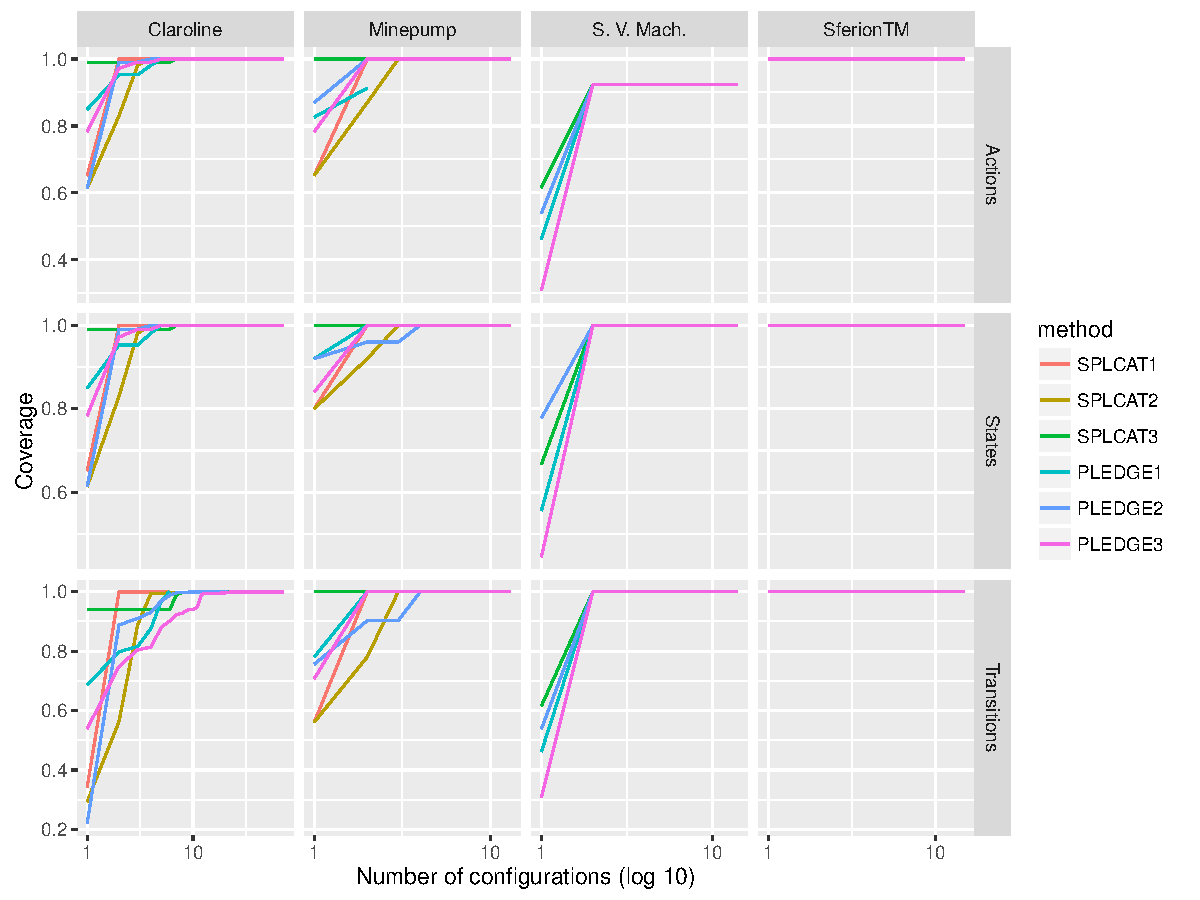
\includegraphics[width=1\textwidth]{configurations-coverage}
	\caption{Behavioural coverage of products selected using SPLCAT and PLEDGE tools}
	\label{fig:behavcov:results}
\end{figure}

Figure \ref{fig:behavcov:results} presents the accumulate behavioural coverage in terms of actions, states, and transitions of the products selected using SPLCAT and PLEDGE. 
%
Results for the soda vending machine exhibit the same tendencies as those of the Minepump. The Sferion\texttrademark landing symbology function has a coverage of $100\%$ for states, transitions, and actions for every product sampled using SPLCAT and PLEDGE, because its FTS has only 4 transitions specific to 2 different features, 2 transitions for each feature, present in each product.
%
Although the number of selected products is higher (as shown in Table \ref{tab:behavcov:toolsparams}), in general, the cumulated coverage value did not increase further after 7 products for states and actions coverage and 14 products for transitions coverage.

%----------------------
\subsection{Discussion}
%----------------------

Regarding our research question, for the considered case studies and settings, we rapidly obtain a complete coverage: relatively few products are needed to fully cover states, transitions, and actions for the two tools reported here. This is to be expected for our small case studies, but on a larger model (Claroline), this tendency tends to be confirmed. Of course, this assessment need to be replicated on a larger sample of behavioural models, but this seems encouraging for the usage of structural coverage criteria at the feature model level beyond the scope of detecting behavioural feature interactions \cite{Cichos2011}. 

On the small feature models, exact $t$-wise coverage (SPLCAT) yields better coverage on all our behavioural criteria for $t=3$. This further indicates that higher values than the usual 2-wise are relevant \cite{Steffens2012} and therefore should be used when the number of products is reasonable. PLEDGE tends to outperform  SPLCAT on 1-wise (each feature is covered at least once) and 2-wise with a smaller number of products. Since for a given execution time, a smaller number of products means more time to  evolve the population (set of products) and less time spent computing distances amongst them, maybe the poor performance of PLEDGE for $t=3$, the largest number of products, can be explained in such a way. We also use the local maximum distance  (called \textit{greedy} in the tool), which is outperformed in terms of coverage by the global maximum distance (called \textit{NearOptimal} in the tool) \cite{Henard2014}. It also  seems that some of the memory errors we run into (related to thread creation) can be accounted by this default choice of the algorithm. Indeed, threads are associated to evolutions of the population and local distance algorithm is fast: we therefore have a thread explosion problem on these small feature models. Therefore, additional settings and trade-offs need to be investigated to be able to compare the tools. Detailed tool comparison in this context is beyond the scope of our research question and is therefore left for future work.

Finally, for both approaches, this initial assessment shows that there is also a need for prioritisation and optimal behavioural coverage. For example, amongst the 71 products selected by SPLCAT ($t=3$), only one is sufficient to cover all states on both the Minepump and Claroline models. This product can be found directly using the all-states coverage test case selection algorithm and the p-coverage upper bound property. If dissimilarity and \textit{t}-wise coverage are shown to consistently sample products that achieve good behavioural coverage, as this assessment suggests, then they can be used as first filters on very large feature models (assuming an intractable FTS for a test case selection algorithm) to prune the FTS and then perform a behavioural coverage driven test case selection. Prioritisation may be initiated at the FTS level and combined with behavioural/structural criteria. There is no such one-criteria-fits-all approach in this endeavour: an all-states criterion may poorly cover transitions (\eg on the Claroline case).  Exploring synergies between these criteria, both at the structural and behavioural models, therefore seems the best option.   


%--------------------------------
\subsection{Threats to validity}
%--------------------------------

%\paragraph{Construct validity:}
%----------------------------

The PLEDGE input parameters are arbitrarily chosen. To keep a fair comparison between the results of the PLEDGE and SPLCAT tools, we keep the same number of products $x$ as sampled by SPLCAT. Estimating the time $d$, however is more tricky. In their comparison, Henard \etal \cite{Henard2014} use the same sampling time as SPLCAT. Unfortunately in our case, some \textit{t}-wise computations take less than 1 second in SPLCAT and PLEDGE does not allow to enter such values. Thus we initially went for the default values provided by the tool. As mentioned above, playing with a wider range of parameter values and with different similarity algorithms will mitigate this threat.

FTS models relate variability to behaviour using feature expressions on transitions, other modelling languages may relate variability to behaviour in other ways (\eg associate variability to states instead of transitions), which will give different results for the state, transitions and actions coverage. FTS is a basic formalism to which we can easily transform other modelling languages and mappings. Thus, we can investigate the influence of the mapping between features and behavioural models.    

%\paragraph{External validity:}
%%----------------------------
%
%We cannot guarantee that our 4 models are representative of real SPLs. We mixed sources and domains to mitigate this threat. 
%The small number of features in the considered feature model does not allow us to generalize our results for large product lines. To the best of our knowledge, there exists no feature model with both a large number of features and an associated behavioural model accessible for research and experimentation.


%%%%%%%%%%%%%%%%%%%%%%%%%%%%%%%%%%%%%%%%%%%%%%%%%%%%%%%%%%%%%%%%%%%%%%%%%
\section{Usage selection and prioritization criteria}
%%%%%%%%%%%%%%%%%%%%%%%%%%%%%%%%%%%%%%%%%%%%%%%%%%%%%%%%%%%%%%%%%%%%%%%%%

\label{sec:experiment:usage}

In this section,  we report on the \emph{feasibility} of using family-based test selection \cite{Devroey2014,Devroey2015a} by applying it on two systems: the first one is Claroline (see section \ref{sec:casestudy:claroline}), and the second one is the landing symbology function, part of Sferion\texttrademark (see section \ref{sec:casestudy:sferion}). Validation of the product-based test selection has been done by Samih \etal \cite{Samih2014}.
%
We assess the feasibility of our approach using the following research questions:
\begin{itemize}
\item \textbf{\textit{FTS pruning} (RQ.1) } What are the reductions gains (model pruning) achieved by applying statistical  prioritization?    
\item \textbf{\textit{Modelling} (RQ.2) } What is the modelling effort induced by our approach and what are the consequences of modelling choices?
\item \textbf{\textit{Scalability} (RQ.3) } How does prioritization scale to increasing probability ranges and what are the implications for testing?  
\end{itemize}

It is difficult to provide precise thresholds for these criteria. Testing should fit a given budget, which is a complex trade-off involving testing time, human and infrastructure resources, level of system coverage desired, \etc  Statistical approaches covered in this thesis are  flexible to meet such a tradeoff. We argue that fixing meaningful  thresholds values requires additional experience, especially in industrial settings where they both can be set and assessed. We therefore leave this issue for future work, giving both quantitative and qualitative information stemming from our experience applying our techniques on Claroline and Sferion\texttrademark.    

%-----------------------------------------------------------
\subsection{Claroline, an online course management system}
%-----------------------------------------------------------

\paragraph{Setup:}
%----------------

We derived the \gls{usage model}, from the same anonymized Apache webserver log as for Claroline FTS (see section \ref{sec:casestudy:claroline:fts}), using a classical bigram inference technique \cite{Ghezzi2014,Sampath2008,Sprenkle2013}: algorithm \ref{algo:bigram} has been adapted to produce a usage model giving algorithm \ref{algo:bigramusagemodel}. As previously, we consider resource names in the user sessions as states (lines \ref{algo:bigramusagemodel:line:sessioninit1} and \ref{algo:bigramusagemodel:line:addstate}) and add transitions between those names if they appear successively in the user sessions (lines \ref{algo:bigramusagemodel:line:sessioninit4} and \ref{algo:bigramusagemodel:line:addtransition}). To compute the probability of each transition, we count the number of occurrences of the transitions (lines \ref{algo:bigramusagemodel:line:sessioninit5}, \ref{algo:bigramusagemodel:line:incrementtrcount}, and \ref{algo:bigramusagemodel:line:incrementfinaltrcount}) and for each transition, we divide this count by the total number of occurrences having the same source state (lines \ref{algo:bigramusagemodel:line:probaloop} and \ref{algo:bigramusagemodel:line:probadef}).

\begin{algorithm}[t]
	\KwIn{$sessions$: the set of non empty user sessions}
	\KwOut{$um$: a usage model representing a navigational model for the given user sessions}
	\Begin{
		$S = \{ s_0 \}$; $Act = \emptyset$; $trans = \emptyset$; $\tau(s_0) = 1$\; \nllabel{algo:bigramusagemodel:line:init}
		\For{sess $\in$ sessions \nllabel{algo:bigramusagemodel:line:mainloop}}{
			$S.add(sess[0])$\; \nllabel{algo:bigramusagemodel:line:sessioninit1}
			$Act.add(req(sess[0]))$ \; \nllabel{algo:bigramusagemodel:line:sessioninit2}
			$tr = s_0 \xrightarrow{req(sess[0])} sess[0]$\; \nllabel{algo:bigramusagemodel:line:sessioninit3}
			$trans.add(tr)$\; \nllabel{algo:bigramusagemodel:line:sessioninit4}
			$count(tr) = count(tr) + 1$\; \nllabel{algo:bigramusagemodel:line:sessioninit5}
			\For{$i \in [1;sess.size[$ \nllabel{algo:bigramusagemodel:line:sessionloop}}{
				$S.add(sess[i])$\;  \nllabel{algo:bigramusagemodel:line:addstate}
				$Act.add(req(sess[i]))$\; \nllabel{algo:bigramusagemodel:line:addaction}
				$tr = sess[i-1] \xrightarrow{req(sess[i])} sess[i]$\; 
				$trans.add(tr)$\; \nllabel{algo:bigramusagemodel:line:addtransition}
				$count(tr) = count(tr) + 1$\; \nllabel{algo:bigramusagemodel:line:incrementtrcount}
	  		}
			$Act.add(req(s_0))$\; 
			$tr = sess[sess.size - 1] \xrightarrow{req(s_0)} s_0$\;
			$trans.add(tr)$\;	 \nllabel{algo:bigramusagemodel:line:addfinaltransition}
			$count(tr) = count(tr) + 1$\; \nllabel{algo:bigramusagemodel:line:incrementfinaltrcount}
	  	}
		\For{$(s_k \xrightarrow{\alpha_i} s_l) \in trans$ \nllabel{algo:bigramusagemodel:line:probaloop}}{
			$P(s_k \xrightarrow{\alpha_i} s_l) = \dfrac{count(s_k \xrightarrow{\alpha_i} s_l)}{\sum_{(s_k \xrightarrow{\alpha_j} s_m) \in trans} count(s_k \xrightarrow{\alpha_j} s_n)} $\; \nllabel{algo:bigramusagemodel:line:probadef}
		}
	  	$um = (S, Act, trans, P, \tau)$\; \nllabel{algo:bigramusagemodel:line:ftsinit}
  		\Return $um$\;
	}
	\caption{Bigram usage model building}
 \label{algo:bigramusagemodel}
\end{algorithm}

The $allpaths$ algorithm has been applied four times to the Claroline usage model with a maximal length ($l_{max}$) of 98 (the maximal path length without any loop in the usage model), a maximal probability ($Pr_{max}$) of $1$, and four different minimal probabilities ($Pr_{min}$), 1e-4, 1e-5, 1e-6, and 1e-7, to observe patterns. Additionally, the algorithm has been parametrized to consider each transition only once (\ie a transition does not appear more than once in a selected trace). This modification has been made since we discovered after a few runs that the algorithm produced a lot of traces with repeated actions, which is of little interest for product prioritization. Repetitions were due to the huge number of loops in the Claroline usage model. 

\paragraph{Results:}
%-------------------

\begin{table}[t]
\centering
\caption{Claroline family-based test selection results}
\label{tab:familybased:claroline}
\begin{small}
\begin{tabular}{lrrrr} 
\hline
	& \textbf{run 1}	& \textbf{run 2}	& \textbf{run 3}	& \textbf{run 4} \\
\hline
$l_{max}$			& 98	 		& 98	  	& 98		& 98 	\\
$Pr_{min}$ 			& 1e-4		& 1e-5 	& 1e-6	& 1e-7	\\
$Pr_{max}$			& 1 	 		& 1	  	& 1		& 1	\\
a.t.c.				& 211 		& 1,389 	& 9,287 	& 62,112	 \\
p.a.t.c. 			& 211 		& 1,389 	& 9,287 	& 62,112 \\
$\overline{size}$ 	& 4.82 		& 5.51 	& 6.35 	& 7.17	\\
$\sigma$ 			& 1.54 		& 1.54 	& 1.62 	& 1.66	\\
$\overline{proba.}$ 	& 2.06e-3 	& 3.36e-4 	& 5.26e-5 	& 8.10e-6	\\
$\sigma$				& 1.39e-2 	& 5.46e-3 	& 2.12e-3 	& 8.18e-4	\\
FTS' st.				& 16 		& 36 	& 50 	& 69	\\
FTS' tr. 			& 66 		& 224 	& 442 	& 844	\\
\hline
\end{tabular}
\end{small}
\end{table}

Results for the four different minimal probabilities are presented in Table \ref{tab:familybased:claroline}.
Execution times range from less than a minute for the first run with 211 abstract test cases (a.t.c) to $\pm 8$ hours for run~4 with 62,112 abstract test cases on a Ubuntu Linux machine (Linux version 3.13.0-65-generic, Ubuntu 4.8.2-19ubuntu1) with an Intel Core i3 (3.10GHz) processor and 4GB of memory.

All abstract test cases selected in the usage model are positive (p.a.t.c.), this is caused by the nature of the Claroline FM: most of the features are independent from each other and few of them have exclusive constraints. The bigram solution used to generate the usage model fits well in this case, as there is no abstract test case selected in the usage model that has been rejected. Sprenkle et al. \cite{Sprenkle2013} experimentally demonstrate that increasing the $n$ in $n$-gram generation of the usage model does increase the size of the generated model in a non linear way (as long as $n$ is between 2 and 10). Increasing the $n$ value in our case would just result in an unnecessary increase of the model complexity.

As expected, the average size of the abstract test cases ($\overline{size}$) increases as the $Pr_{min}$ decrease (a lower probability allows longer traces to be selected). The average size of the user sessions used to generate the usage model is 9.88.

As explained in Algorithm \ref{algo:abstracttestcasesfiltering}, it is possible to prune the original FTS using the positive abstract test cases in order to consider only the valid products capable of executing those test cases. In this case, it eventually reduces the number of states (FTS' st.	) and transitions (FTS' tr.) from 106 and 2,055 (resp.) to 16 and 66 (resp.) in run~1 and to 69 and 844 (resp.) in run~4. As expected, by controlling the interval size we can reduce the number of traces to be considered and yield easily analysable FTS'.


%-------------------------------------------------------------
\subsection{Sferion\texttrademark landing symbology function}
%-------------------------------------------------------------

\paragraph{Setup:}
%-------------------

Engineers will probably have to run the algorithm several times using different minimal and maximal probabilities intervals in order to refine the selection. In our first attempt, we applied our trace selection algorithm 10 times with a maximal probability value of 1 and a minimal probability value ranging from $10^{-1}$ to $10^{-10}$ and a maximal length of $50$. As explained hereafter, some of those runs did not return any relevant results.


\paragraph{Results:}
%-------------------

\begin{table}[t]
\centering
\caption{Sferion\texttrademark landing symbology function family-based test selection results}
\label{tab:familybased:sferion}
\begin{small}
\begin{tabularx}{8.5cm}{lrrrrr} 
\hline
	& \textbf{run 1}	& \textbf{run 2}	& \textbf{run 3}	& \textbf{run 4}	& \textbf{run 5} \\
\hline
$Pr_{min}$ 			& 1e-1	& 1e-2	& 1e-3	& 1e-4	& 1e-5	\\
$Pr_{max}$			& 1	& 1	  & 1	& 1	& 1	\\
a.t.c.				& 0 & 0 & 8 	  & 50 & 306  	\\
p.a.t.c.  			& 0 & 0 & 8 & 50 & 306 	\\
$\overline{size}$	& 0 	& 0 	& 15 	& 16.68 	& 18.58 \\
$\sigma$				& 0	& 0	& 0.76	& 1.17		& 1.39		\\
$\overline{proba.}$	& 0 	& 0 	& 2.19e-3 	& 5.67e-4 	& 1.19e-4 \\
$\sigma$				& 0	& 0	& 1.51e-3	& 9.30e-4	& 4.23e-4	\\
FTS' st.				& 0	& 0	& 18	& 23	& 23	\\
FTS' tr. 			& 0	& 0	& 12	& 12	& 12	\\
FTS' act. 			& 0	& 0	& 27	& 40	& 42	\\
\hline
\end{tabularx}
\end{small}

\vspace{1em}

\begin{small}
\begin{tabularx}{8.5cm}{lrrrrr} 
\hline
	& \textbf{run 6}	& \textbf{run 7}	& \textbf{run 8}	& \textbf{run 9}	& \textbf{run 10} \\
\hline
$Pr_{min}$ 			&  1e-6	& 1e-7	& 1e-8	& 1e-9	& 1e-10	\\
$Pr_{max}$			&  1	& 1	& 1	& 1	& 1	\\
a.t.c.				& 1870 & 8622 & 36582 & 123534 & err 	\\
p.a.t.c. 			& 1870 & 8622 & 36582 & 123534 & err \\
$\overline{size}$	& 20.85 	& 22.99 	& 25.15 	& 27.17	& err 	\\
$\sigma$ 			& 1.62		& 1.77		& 1.88		& 1.97	& err	\\
$\overline{proba.}$	& 2.20e-5 	& 5.02e-6 	& 1.21e-6 	& 3.59e-7 	& err \\
$\sigma$ 			& 1.76e-4	& 8.25e-5	& 4.01e-5	& 2.18e-5	& err 	\\
FTS' st.				& 23	& 23	& 23	& 23	& err	\\
FTS' tr. 			& 12	& 12	& 12	& 12	& err	\\
FTS' act. 			& 42	& 42	& 42	& 42	& err	\\
\hline
\end{tabularx}
\end{small}
\end{table}

The results of the execution are showed in table \ref{tab:familybased:sferion}. The run~10 did not return any results due to the too wide range of considered probabilities, giving too many possible paths in the usage model. This is not a problem for our approach as a wide range of probabilities is not very useful for prioritization. According to those results, the interval with the most probable abstract test case is between 1e-3 and 1e-2. We re-run the algorithm with the minimal probabilities 5e-3 and 2.5e-3: the execution with an interval between [0;5e-3] returned no test case; the execution with an interval between [0;2.5e-3] returned 2 test cases (\textit{test case 1} and (\textit{test case 2})) with an average probability of 4.62e-3 and a length of 14. Those two abstract test cases are the most probable behaviours of the landing symbology function and may be executed by all the products of the product line.

In order to get a more concrete product, we select longer abstract test cases from the usage model by using the classical state-coverage criterion\cite{Mathur2008}. This criteria specifies that, when executing a test suite on the system, all the states of the system have to be visited at least once. Generating an abstract test case from the usage model using this criteria gives us one abstract test case visiting all states (\textit{test case 3}). As for previously selected abstract test cases, we execute it on the FTS to ensure that there exists at least one product able to exercise this behaviour: this gives us a set of 64 products.


%------------------------
\subsection{Discussion}
%------------------------

We organise our discussion on the final results regarding feasibility for statistical prioritization SPL testing according to the criteria mentioned above:
\begin{inparaenum}[(i)]
\item FTS pruning; 
\item modelling; and 
\item scalability.
\end{inparaenum}


\paragraph{FTS pruning (RQ.1):}  
%-----------------------

In both cases, it was possible to substantially prune the FTS  models according to frequent behaviours: from 28\% to 85\% reduction \wrt the number of states (for Sferion\texttrademark and Claroline)  and up to 99,994\% reduction \wrt to transitions (for Claroline).  These important reduction factors are interesting in the sense that it is possible to use statistical selection to deal with additional computationally expensive coverage criteria that would not be directly applicable on the original model (\eg  all-paths coverage on the Claroline FTS \cite{Devroey2014c}). 

Regarding the number of products associated with the selected test cases, the situation is less favourable.  In the Claroline case, the least probable test case in run 1 is already associated to 260 products. The main reason is that test cases are small in size yielding short associated feature expressions. Most Claroline users therefore seems to visit few pages after the login one. Because the source Apache Log is anonymised, it is impossible to investigate further in this direction. To note that the set of 260 products is reduced to 20 products if we consider only courses available to student with an id, which is the most classical scenario in the University of Namur Claroline instance. The tester will have to use his knowledge of the application domain in order to reduce the number of products to test. 

The Symbology function exhibits more complex behaviours as witnessed by test cases' sizes.  For Sferion\texttrademark, there are test cases that can be executed by all the products of the SPL. While from pure product selection perspective this is a bad result, two additional observations need to be made. First,  the usage model was provided by experts to focus on the most relevant behaviours: it seems they did perform correctly this task as most part of the described behaviour concern all the products of the SPL. Second, there are opportunities to reuse abstract test cases amongst products: these two abstract test cases can be used to derive a small number of concrete test cases covering all products. This strategy can be used to explore interaction problems \cite{Nguyen2014}. Finally, feature models of our considered systems have very few constraints (\eg $Mark\_landing\_position \Rightarrow HOCAS$, $Check\_for\_obstacles \Rightarrow OWS$, \etc) amongst features, which clearly influence product reduction ability. While such  an open feature model is not surprising for a web based system, this is more unusual for an embedded SPL.                 

\paragraph{Modelling (RQ.2):}
%---------------------

Using statistical prioritisation in both case studies involved some modelling: the family-based scenario allowed us to extract automatically the usage model using a machine learning technique, while the Sferion\texttrademark product one relied on SPL and testing experts to explicitly provide the required usage model. However, what is common to both scenarios is the necessity to provide variability models (in OVM or TVL)  and mapping from features to behaviours either by means of FTS or mapping matrices \cite{Samih2014b,Samih2014}. 

Both approaches try to keep requirements from test models separated. Such a separation of concerns does not guarantee that these models are correct (learning behaviours from anonymous logs entails approximations and hand-made usage model are not free from biases either)  but helps finding discrepancies as they are generally provided by stakeholders having different perspectives and skills. Keeping these models separated was also useful to integrate our approach with tools like MaTeLo that do not take into account natively features in their usage models but provide additional facilities such as risk management or customer satisfaction during test case selection.

Separation of the usage model from the FTS also allows to use different usage models, depending on the objective of the test engineer. For instance, Claroline has a fine grained access control system. In its basic setup, it comes with three user roles: Administrator, Teacher and User. According to its role, a user may or may not perform different actions and access different functionalities. Claroline also allows public access to some pages and functionalities (\eg a course description) to anonymous users. We think that since those four user roles have very different usage profiles, a better approach would be to create four different usage models, one for each user role. Unfortunately, it was not possible in our case with the provided Apache access log since the user roles have been erased in the anonymisation process.

Keeping the usage model and the FTS separated may be detrimental to the analysis as some invalid abstract test cases may be first extracted from the usage model and then removed. Even if this was not the case on the considered SPLs, this may happen in more constrained SPLs. One strategy could be to start with separated models and to merge them in a feature-aware usage model (\eg using feature-aware discrete-time Markov chain \cite{Rodrigues2015,terBeek2016}) once enough confidence is gained on both models. This is left for future work.

The effort spent in modelling activities depends on the case study: for the Claroline case study, the usage model has been automatically generated, the FTS has been semi-automatically generated and the variability model has been hand crafted. Given the size of Claroline (442.399 LOC), the total effort spent in modelling activities is deemed reasonable (around 7 days). The Sferion\texttrademark case study models a critical system, the modelling and testing efforts are important but have to be supported by the company in order to guaranty a safe and sound product. The additional effort required to derive the FTS from the Sferion\texttrademark models is small (around 2 days).


\paragraph{Scalability (RQ.3):}
%-----------------------

Final results show that the scalability of our implementation mainly depends on the $[Pr_{min}, Pr_{max}]$ interval and the shape of the usage model. We notice that if the model is large (Claroline)  and/or the probability  interval very large computation time obviously increases and may even lead to no result at all  (\eg run 10 in Table \ref{tab:familybased:sferion}). In this case we encountered memory overflows. The \emph{allpaths} algorithm used in our implementation seems to perform well as long as the $[Pr_{min}, Pr_{max}]$ interval is not too wide, even on large usage model (like the Claroline case). Thus, we rely upon the tester to choose a relatively small probability interval in order to extract behaviours that results in the desired amount of test cases and products. So far, we explored these intervals manually to find tradeoffs. This exploration can be automated if additional criteria (such as the maximum number of products desired) are specified. Other state space exploration techniques will have to be investigated to improve the algorithm (\eg limit the length of the selected test cases is amongst the simplest, or use simulation techniques \cite{Baier2008}). It should be noted that, for more specialized explorations, such as finding the most probable path, dedicated algorithms like the one proposed by Viterbi \cite{Viterbi1967} may be used.    


%---------------------------------
\subsection{Threats to validity}
%---------------------------------


%\paragraph{Construct validity:}
%------------------------------

To implement our approach, we choose to use a \emph{allpaths} algorithm with some restrictions (maximal length of the selected test cases) in order to avoid infinite executions. This choice may be not optimal but the \emph{allpaths} exploration ensure (in worst case) a complete exploration of the usage model. The input models (DTMC as a usage model, FTS and TVL) are not the only possibilities to represent usages, behaviour, and variability of the SPL. In our second SPL, we showed how we translate other input models in order to apply our approach.

%\paragraph{External validity:}
%%-----------------------------
%
%The main threat is the nature of the considered applications as it influences the shape of the different models: average degree in the FTS and usage model, number of features in the FM, number and nature of the constraints in the FM, \etc The first considered system is a very particular kind of application: a web application accessible through PHP pages in a web browser with a small number of states and a huge number of transitions. This kind of application allows a very flexible navigation from page to page either by clicking on the links in the different pages or by a direct access with a link in a bookmark or an e-mail for instance. In order to mitigate this risk, we applied our approach to the Sferion\texttrademark landing symbology function, an embedded system. The diversity of the considered systems and models gives us a good confidence in the possibilities of generalisation of our approach.



%%%%%%%%%%%%%%%%%%%%%%%%%%%%%%%%%%%%
\section{Mutants execution}
%%%%%%%%%%%%%%%%%%%%%%%%%%%%%%%%%%%%

\label{sec:experiment:fmmexec}

This section reports on our comparison \cite{Devroey2016a} between the \gls{FMM} approach, that uses a compact representation to factorize the mutants execution against each test case, and the enumerative approach, where each mutant is executed individually against each test case, in terms of execution time. And evaluates the usage of \glspl{FMM} to perform higher-order mutation analysis.
As in Section \ref{sec:FMM}, we adopt a product-based strategy: the systems under test, used as original systems to perform the mutation analysis, are products derived from our case studies described in Chapter \ref{chap:casestudies}. In order to conduct this assessments, we formulate our research questions as follows:
\begin{itemize}
\item \textbf{\textit{Execution time} (RQ.1) } How does the FMM scheme compare with the enumerative approach in terms of execution time?
\item \textbf{\textit{Higher-order mutation} (RQ.2) } Is higher-order mutation under the FMM scheme tractable?
\end{itemize}

%----------------------
\subsection{Setup}
%-----------------------

To perform the assessment, we project the FTSs of the case studies described in Chapter \ref{chap:casestudies} to get the original LTSs that will serve as basis for our mutation analysis. We consider products from different sources with varying size. Our models are: 
\begin{itemize}
\item a soda vending machine product (\textit{Soda V. Mach.}) that includes all features;
\item a Minepump product (\textit{Mine\-pump}) that includes all features;
\item a Claroline product (\textit{Claroline}) that includes all features and an \textit{Admin} user;
\item three WordPress products (\textit{AGE-RR}, \textit{Elsa-RR}, and \textit{Elsa-RRN}) that include all features of their respective feature models
\item one random model (Random 1).
\end{itemize}

\paragraph{Test cases:} 
%----------------------

\begin{table}
\centering
\caption{Test suites characteristics}
\begin{small}
\begin{tabular}{l r r r r r}
\hline
\textbf{Model}	& \multicolumn{2}{c}{\textbf{Random test suite}}	& \multicolumn{3}{c}{\textbf{All-actions test suite}}	\\
	& \textit{$\overline{size}$} & \textit{$\sigma$}	& \textit{count} & \textit{$\overline{size}$} & \textit{$\sigma$}	 \\
\hline 
Soda~V.~Mach.	& 4.78 	& 1.34 	& 3 		& 5.33 	& 2.08 \\
Minepump			& 5.65 	& 1.23 	& 9 		& 6.11 	& 1.45 \\
Claroline		& 17.11 	& 16.97 	& 11 	& 13.18 	& 9.20 \\
AGE-RR			& 21.13 	& 24.58 	& 274 	& 27.11 	& 33.62 \\
Elsa-RR			& 10.57 	& 13.12 	& 109 	& 21.10 	& 33.45 \\
Elsa-RRN			& 10.45 	& 14.05 	& 148 	& 23.20 	& 43.49 \\
Random 1 			& 469.62	& 279.34	& 2 		& 468.50	& 118.09 \\
\hline
\end{tabular}
\end{small}
\label{tab:experiment:fmmexec:testsets}
\end{table}

For each model, we select one test suite using random walks on the LTS and one test suite satisfying the all-actions criterion.
The test suites are then executed with the enumerative and the FMM processes. Table \ref{tab:experiment:fmmexec:testsets} records the average size (and standard deviation) of the randomly selected test cases, the size of the selected all-actions coverage-driven test suite and the average size (and standard deviation) of its test cases. The size of the random test suite is arbitrarily fixed to 100 test cases. 

\paragraph{Model mutants:}
%-------------------------

\begin{table}[t]
\centering
\caption{Mutants count per operator}
\begin{small}
\begin{tabular}{l r r r r r r r r}
\hline
\textbf{Model}	& \textbf{WIS}	& \textbf{TMI}	& \textbf{AEX} & \textbf{TDE}	& \textbf{TAD} & \textbf{AMI} & \textbf{SMI} & \textbf{Total}\\
\hline 
Soda~V.~Mach.	& 1		& 1		& 1	& 1		& 1	& 1	& 1	& 7 \\
Minepump			& 2		& 4		& 4	& 4		& 4	& 3	& 2	& 23 	\\
Claroline		& 9		& 188	& 205	& 204		& 205	& 189	& 9	& 1,009	\\
AGE-RR			& 73		& 525	& 663 	& 663		& 663	& 516	& 75	& 3,178 \\
Elsa-RR			& 36		& 102	& 121	& 121	& 121	& 106	& 38		& 645 \\
Elsa-RRN			& 57		& 153	& 177	& 177	& 177	& 155	& 57		& 953 \\
Random 1 			& 942	& 1,276	& 1,365 	& 1,365	& 1,365 & 1,295 & 954 	& 8,562 \\
\hline
\end{tabular}
\end{small}
\label{tab:experiment:fmmexec:mutants}
\end{table}

We used the operators presented in Annex \ref{apdx:fmm:operators}. Operators modifying states (WIS and SMI) or transitions (TMI, AEX, TDE, TAD, and AMI), respectively, were applied arbitrarily for 1/10 of the number of states or transitions, respectively, in the model (with 1 as bottom value). Since the operands are randomly chosen, we forbid multiple applications of any operator on the same operands to avoid duplicated mutants \cite{Papadakis2015}. Table \ref{tab:experiment:fmmexec:mutants} presents the number of mutants generated per operator for the studied models.


\paragraph{Mutants execution:}
%----------------------------

To avoid execution time bias from the underlying machines, we execute each test case 3 times with each considered mutant (for the enumerative version) and on the FMM. Experimentation was performed on an Ubuntu 14.04 LTS Linux (kernel 3.13) machine with Intel Core i3 (3.10GHz) processor and 4GB of memory. The complete experiment took approximately 2 weeks.

%----------------------
\subsection{Results}
%----------------------

\begin{figure}
	\centering
	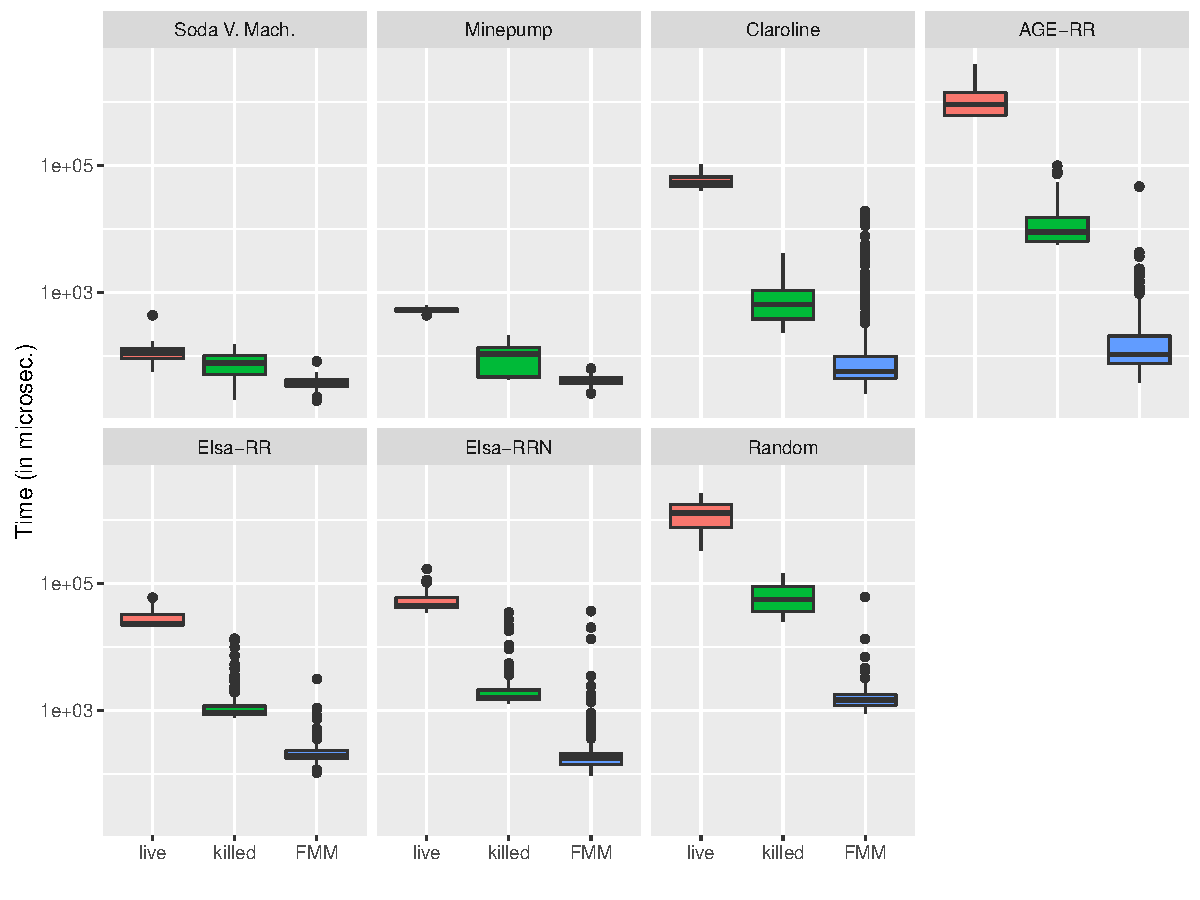
\includegraphics[width=0.98\textwidth]{mutants-exec-time}
	\caption{Execution time required by test cases to executed with live and killed mutants and the FMM mutants}
	\label{fig:assessment:mutantsexectime}
\end{figure}

Figure \ref{fig:assessment:mutantsexectime} presents the distribution of the test execution time (in logarithmic scale on the \textit{y} axis) for each studied model with a box plot. The first two columns represent the total execution time taken by each test case when executed on the live mutants and on the killed mutants according to the enumerative approach. The third box presents the execution time of the FMM (FMM approach). Note that while the killed mutants do not require a complete execution in the enumerative approach, it is required for the FMM mutants. This might provide an advantage to the enumerative approach. To assess this, we consider the killed and the live mutants separately. In all cases, we measure only the execution of the models, avoiding time bias due to I/O operations.
As the execution time of a test case partially depends on its size, the high number of outliers in Figure \ref{fig:assessment:mutantsexectime} is explained by the variation of the test cases sizes.

For the enumerative approach, executing a test case on mutants that will remain live takes more time than executing the same test cases on mutants that are killed. This was expected since killed mutants do not require a complete execution of the test case.
In both cases, the FMM execution runs faster, \ie running a test case on all the mutants at once is very fast, despite the more complex (needed) exploration of the FMM's FTS. Detailed statistics over the execution time of the models and mutation scores are presented in Annex \ref{apdx:fmm:exectime}. 

%----------------------
\subsection{Discussion}
%----------------------

\paragraph{Execution time:}
%--------------------------

Regarding \emph{RQ1}, the box plots of Figure \ref{fig:assessment:mutantsexectime} (and the values in Annex \ref{apdx:fmm:exectime}) confirm that the execution time required by the FMM approach is considerably lower than the time required by the enumerative approach. The difference escalates to several orders of magnitude when considering live mutants. The difference between family-based and enumerative approaches increases with the size of the model, indicating the improved scalability of our approach.

To evaluate the statistical significance, we use a Wilcoxon rank-sum test for the different models we considered: we obtain a $p$-value of $1.343e-09$ for the random model and $p$-values smaller than $2.2e-16$ for the other models, confirming the hypothesis that FMM significantly outperforms the enumerative approach, when considering $0.001$ significance level. 

\paragraph{Higher-order mutation:}
%---------------------------------

\begin{table}
\centering
\caption{All-order mutation scores}
\begin{small}
\begin{tabular}{l rrrrrrr}
\hline
\textbf{Model}	& \textbf{\# mutants}	& \multicolumn{3}{c}{\textbf{All-actions}}	& \multicolumn{3}{c}{\textbf{Random}}\\
	& 	& \textit{\#Lv.}	& \textit{MS} & \textit{Time}	&  \textit{\#Lv.}	& \textit{MS} & \textit{Time}	 \\
\hline 
Soda V. Mach.	&	127						& 1			& 0.99 & 1.10  & 1 & 0.99 & 17.67 \\
Minepump		&	8,388,607					& 1			& >0.99	& 1.84 & 1	& >0.99 & 15.72 \\
Claroline	&	5.49e+303	& \multicolumn{3}{c}{Timeout} & \multicolumn{3}{c}{Timeout} \\
AGE-RR		&	4.71e+956	 				& \multicolumn{3}{c}{Timeout} & \multicolumn{3}{c}{Timeout} \\
Elsa-RR		&	1.46e+194	& 2916	& >0.99	& 37.78  &  144	& >0.99 & 10.19 \\
Elsa-RRN		&	7.61e+286	& 36			& >0.99	& 150.32  & 16		& >0.99 & 83.04 \\
Random 1		&	2.62e+2577					& \multicolumn{3}{c}{Memory overflow} & \multicolumn{3}{c}{Memory overflow} \\
\hline
\end{tabular}
\end{small}
\label{tab:experiment:fmmexec:norderscore}
\end{table}

Table \ref{tab:experiment:fmmexec:norderscore} presents the number of all-order mutants for our models, the number of mutants live after executing the random and all-actions test sets (computed using SAT4J 2.3.5), and their mutation score. For each test set and model, the table records the number of possible mutants (\textit{\# mutants}), the number of live mutants after the test set execution (\textit{\#Lv.}), the mutations score (\textit{MS}) and the SAT computation time (\textit{Time}) in seconds. \textit{Memory Overflow} denotes an overflow during SAT solving, improving this step by, for instance, reducing the boolean formula to process is part of our future work. Columns 5 and 8 give the SAT-solving computation time (we set a timeout of 12 hours). 

Overall, our results suggest that higher-order mutation under the FMM scheme is tractable, answering positively to \emph{RQ2}.  In particular, all-order mutation achieves very good mutation scores ($MS \geq 0.99$) when compared to first-order mutation when this score can be computed. In our future work, we intend to: improve the scalability of mutation score computation; and assess the practical relevance of higher-order in test sets comparison.

Only one mutant is live for the soda vending machine and the Minepump products. This mutant is a first order mutant resulting from the TAD operator. Indeed, the TAD operator adds new transition which cannot be detected by test cases solely selected from the original LTS, since this transition does not exist in this model. All-order mutation enables to quickly kill mutants of any order an to focus on the interesting ones from a selective mutation perspective. For example, the 2,916 remaining live mutants resulting from the execution of the all-action test suite are relevant to study the mutation operators involved. Of course, they can also be used to select test cases killing them in order to augment the test suite. Exploring all-order mutation score in selective mutation or test case selection scenarios are part of our future work.  

%----------------------------------
\subsection{Threats to validity}
%----------------------------------

%\paragraph{Construct validity:}
%------------------------------

We chose to apply mutants for $1/10$ of the states and/or transitions of the mutated model. This might result in more (or less) mutants than needed for the larger models. However, this is expected when using mutation. Additionally, since model-based mutation is applied to the system's abstraction, abstract actions represent many concrete actions. It is therefore important to ensure a good coverage of most of the model actions.

TS and FTS executions are different, and do not use the same algorithms. In order to decrease the bias in measuring execution time, both executions of the models have been done using VIBeS, our \emph{Variability Intensive Behavioural teSting framework} Java implementation. The two execution classes are different but use a variant of the same algorithm described in Section \ref{sec:FMM}. Moreover, we used the \texttt{Stopwatch} Java class to measure the call to the execute method (\ie model loading and result writing time have been omitted). 
Finally, we ran each test case 3 times on each mutant model (LTSs and FMMs) to avoid bias due to process concurrency.

%\paragraph{External validity:}
%%------------------------------
%
%We cannot guarantee that our results are generalizable to all behavioural models. However, we recall the diversity of the model sources (hand-crafted, reverse-engineered, and randomly generated to match real system state-space) as well as the diversity of considered systems.


%%%%%%%%%%%%%%%%%%%%%%%%%%%%%%%%%%%%
\section{Mutant equivalence analysis}
%%%%%%%%%%%%%%%%%%%%%%%%%%%%%%%%%%%%

\label{sec:experiment:mutequiv}
% apdx:fmm:equivalence

\glsreset{ALE} \glsreset{RS} \glsreset{BS}  \glsreset{WM} \glsreset{SM}  

This section presents our empirical assessment of the \gls{ALE}, \gls{RS}, and \gls{BS} approaches to detect equivalent mutants \cite{Devroey2017}. As in Section \ref{sec:EMP}, we adopt a product-based strategy: mutants are generated from products, derived from the case studies defined in Chapter \ref{chap:casestudies} (and from 4 additional randomly generated models). To conduct this assessment, we define the following research questions:
\begin{itemize}
\item \textbf{\textit{Random/biased simulations and ALE} (RQ.1) } What is the impact of weak and strong mutation on BS/RS \textit{vs}. ALE performance?
\item \textbf{\textit{Non-equivalent mutant detection} (RQ.2) } How many non-equivalent mutants are effectively detected by the RS and BS appro\-aches?
\item \textbf{\textit{Worst case scenario} (RQ.3) } What are the worst case execution times for the ALE and BS/RS approaches?
\end{itemize}

%----------------------
\subsection{Setup}
%-----------------------

To answer these RQs, we consider several models of different kinds of systems and apply the following procedure to each of them:
\begin{enumerate}
\item we generate a set of mutants from the model using the operators presented in Annex \ref{apdx:fmm:operators} for orders 1, 2, 5, and 10;
\item for each order, we sample 100 non-equivalent mutants (using the ALE algorithm to guarantee non-equivalence) to form the mutant set $M$;
\item for each mutant in $M$, we measure the execution time and result of: 3 executions of weak mutation random and biased search (WM RS/BS), and 3 executions of strong mutation-biased search (SM BS) algorithms\footnote{As explained in Section \ref{sec:EMP}, SM RS is not considered for the assessment due to the poor results during our initial attempts.} with 4 different values of $\delta$ and $\epsilon$; and the executions of the ALE algorithm.
\end{enumerate}
In the following we detail the different steps of the procedure. The assessment has been performed on a Debian 3.16.7 x86\_64 GNU/Linux running on a 16 cores, 2.2 GHz, 16Gb RAM virtual machine.

\paragraph{Models:}
%------------------

We carry out the assessment on 12 different models coming from different sources and with varying size. The models are:
\begin{itemize}
\item a soda vending machine product (\textit{S. V. Mach.}) that includes all features;
\item a card payment terminal product (\textit{C. P. Term.}) that includes all features;
\item a Minepump product (\textit{Mine\-pump}) that includes all features;
\item a Claroline product (\textit{Claroline}) that includes all features and an \textit{Admin} user;
\item four WordPress products (\textit{AGE-RR}, \textit{AGE-RRN}, \textit{Elsa-RR}, and \textit{Elsa-RRN}) that include all features of their respective feature models;
\item four random models (Random 1-4).
\end{itemize}

\paragraph{Mutant generation and sampling:}
%-----------------------------------------

First-order mutants are generated using the operators presented in Annex \ref{apdx:fmm:operators}. Each operator is applied (arbitrarily) 10 times on the \textit{S.\-V.\-Mach.}, \textit{C.\-P.\-Term.}, and \textit{Mine\-pump} products. Due to the small size of the models, applying the same mutation operator more than 10 times is not relevant. Operators are also applied (arbitrarily) 500 times on the other models. In the same way, \textit{N}-order mutants (with $N$ equal to 2, 5, or 10 in our case) are generated by applying the same operators 10 or 500 times (depending on the model) on ($N-1$)-order mutants.
After the generation, we perform a random sampling of 100 mutants (when available) for orders 1, 2, 5, and 10, giving us a set $M$ with 370 mutants for the \textit{S.\-V.\-Mach.}, \textit{C.\-P.\-Term.}, and \textit{Mine\-pump} models, and 400 mutants for the other models.
To ease mutant generation, we use the compact representation provided by FMMs. 

\paragraph{Non-determinism:}
%--------------------------

We checked all the 4710 mutants and found that only 3.54\% of them are non-deterministic (\ie there exists a sequence of actions for which there is at least two possible paths in the mutant). Nevertheless, there is a great disparity amongst models as the non-determinism rate varies from 0\% for \textit{Elsa-RRN} to 15.5\% for \textit{Claroline}. Higher-order mutation greatly influenced non-determinism rates: the sole order 10 is responsible for 53\% of all non-deterministic mutants. In terms of mutation operators, TAD accounts for a large majority  of non-deterministic first-order mutants (78\%) and AEX for the remaining 22\%.  At higher orders, these two operators are largely involved. They are absent only in the \textit{Minepump} model where TDE and AMI appear for two non-deterministic mutants. 

\paragraph{Algorithm execution:}
%------------------------------

To run the language equivalence algorithms (for WM and SM), we use the HKC library \cite{hkc}, an OCaml implementation of the ALE  algorithm \cite{Bonchi2013} compiled using OCamlbuild. This tool handles non-deterministic TSs using different strategies: the automata may be processed either forward of backwards, and the exploration strategy may be breadth-first or depth-first. For each mutant, we execute the HKC library using each of the 4 possible configurations. The input models and their mutants have been transformed from our XML format to the Timbuk input format supported by HKC.

The random and biased simulation algorithms are implemented in Java using multi-threading to parallelize trace selection and execution as described in Algorithm \ref{algo:fmm:randomequiv} (lines \ref{line:fmm:randomequiv:posrandomselect}, \ref{line:fmm:randomequiv:posexec}, \ref{line:fmm:randomequiv:negrandomselect}, and \ref{line:fmm:randomequiv:negexec}). In our experiments, we set up the algorithm with 4 threads and run 4 instances in parallel on our virtual machine with 16 cores.
We run the simulation algorithms with 4 different values of $\delta$ and $\epsilon$ determining the number of traces selected and executed ($N$ in Algorithm \ref{algo:fmm:randomequiv}): 
\begin{itemize}
\item RS1/BS1: ($\delta=1e-10$, $\epsilon=0.01$, $N=1,897,519$);
\item RS2/BS2: ($\delta=1e-10$, $\epsilon=0.1$, $N=18,975$);
\item RS3/BS3: ($\delta=1e-5$, $\epsilon=0.1$, $N=9,764$);
\item RS4/BS4: ($\delta=1e-1$, $\epsilon=0.1$, $N=2,396$).
\end{itemize}

For all the simulation configurations and all models, we fixed the trace length $k$ to 3,000, which was our compromise between performance and non-equivalence detection: setting $k$ to BFS height led to crashes in some cases. In order to answer RQ3, we also run each algorithm (RS1/BS1 to RS4/BS4, plus the 4 possible ALE configurations) with the model itself as the mutant. Those (unrealistic) equivalent detection runs between the model and itself are only used to approximate the worst computation time of the different algorithms.

%-----------------------------------
\subsection{Results and discussion}
%-----------------------------------

\paragraph{Random/biased simulations and ALE:}
%--------------------------------------------

\begin{figure}[t]
	\centering
	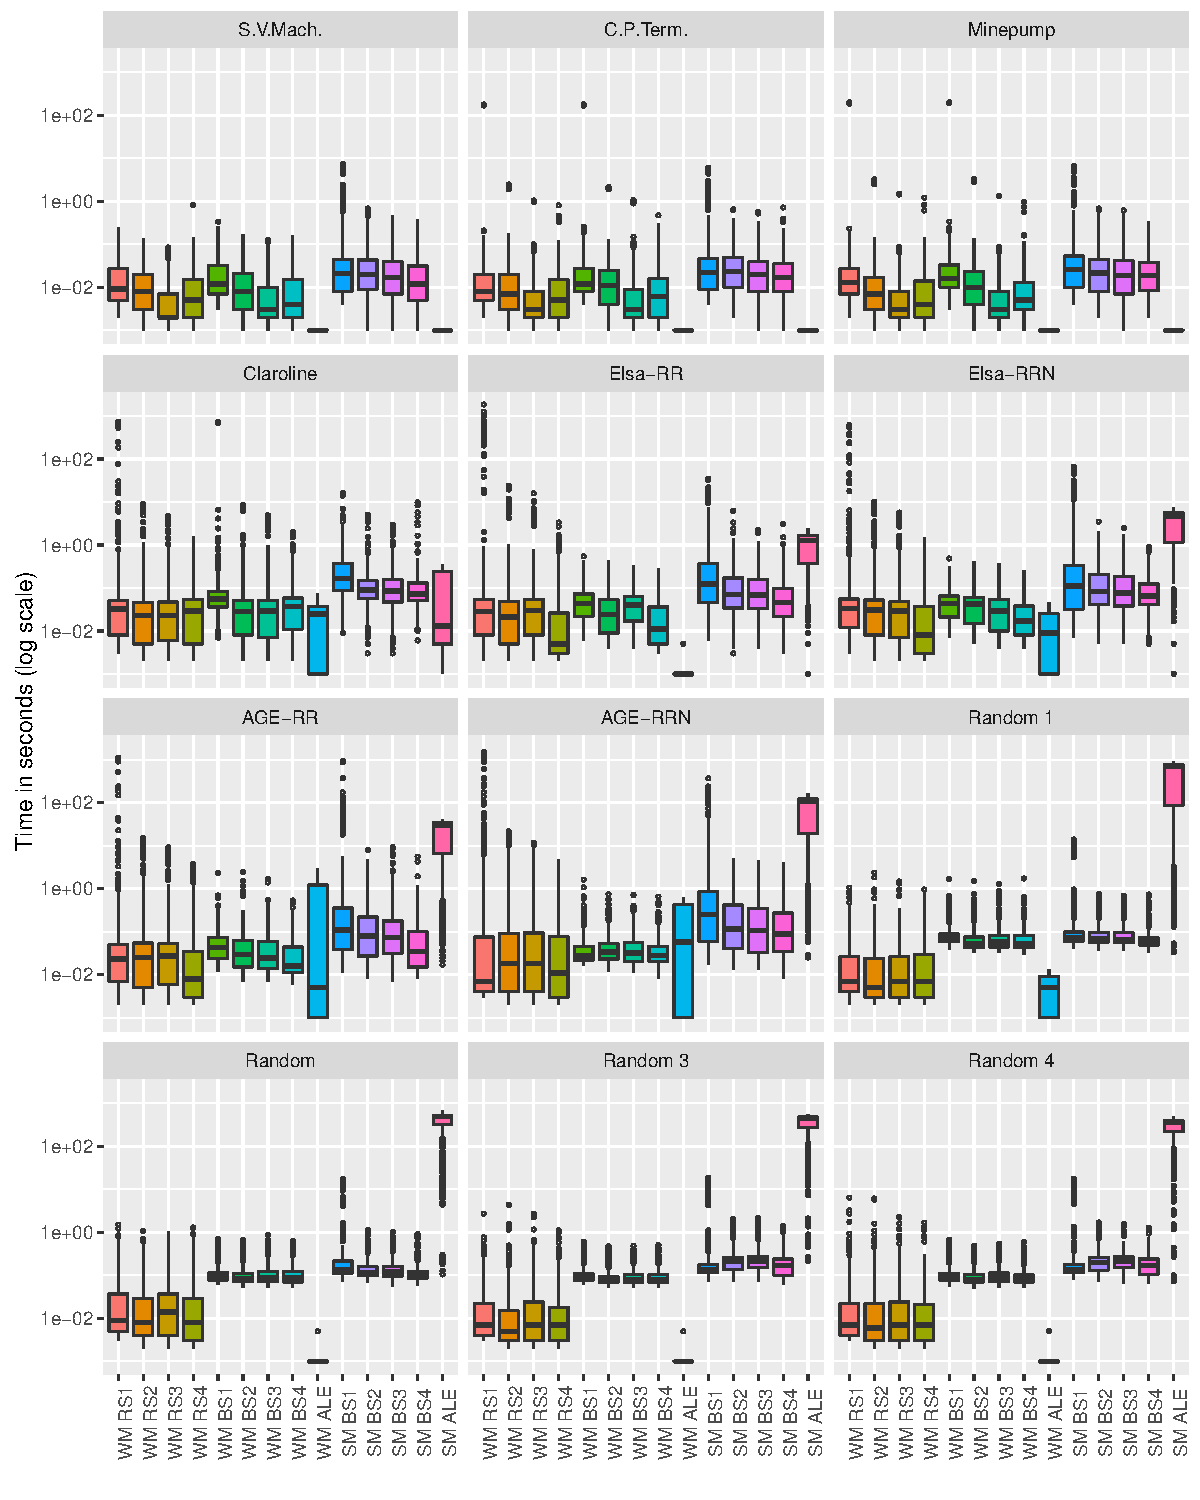
\includegraphics[width=0.98\textwidth]{mutants-equiv-time}
	\caption{Execution time of the equivalent mutant detection approaches}
	\label{fig:assessment:mutantsequivtime}
\end{figure}

Figure \ref{fig:assessment:mutantsequivtime} presents the execution time per mutant of the studied algorithms, which is detailed in the Appendix. Regarding weak mutation scenarios, the ALE approach is the fastest in all cases in eleven of our models. On the \textit{AGE-RN} model,  biased simulations are faster for the largest numbers of runs.  However, the results are at the limit of non-significance (see Table \ref{tab:assessment:mutantsequivwmpvalues}), so that the only clearly significant result is for \emph{BS1} on this model. For \textit{AGE-RNN}, execution times for  biased simulations are non-significant. Random simulations are also faster than ALE on \textit{AGE-RRN} but only certain settings are significant. We thus conclude that the ALE approach is more interesting in terms of execution time. When we compare the two forms of simulations, for the smallest models, biased simulations are either on par for the smallest models or slightly better. Additional computations such as the breath-first search used for biased simulation do not cause significant overhead. For the largest random models, random simulations are faster. In these cases, the overhead of computing infected states and paths that cover these states is greater and random simulation is faster.  However, lower standard deviations for biased simulation execution times over random ones make the BS approach easier to use.
       
Regarding strong mutation, several observations can be made. First, random simulations provide very high execution times compared to biased simulations or the ALE algorithm (the analysis of one model is stopped after one hour). This may be due to the difficulty to reach the initial state again when performing random walks in the TSs.
Second, biased simulations are faster than ALE executions for models larger than 300 states. On the largest models, biased simulations can be up to 1,000 times faster. We thus conclude that these are the most interesting situations in which to use BS, for mutation analysis.  On smaller models, the ALE algorithm's performance is quite impressive and therefore should be privileged.              

\paragraph{Non-equivalent mutant detection:}
%--------------------------------------------

\begin{figure}
	\centering
	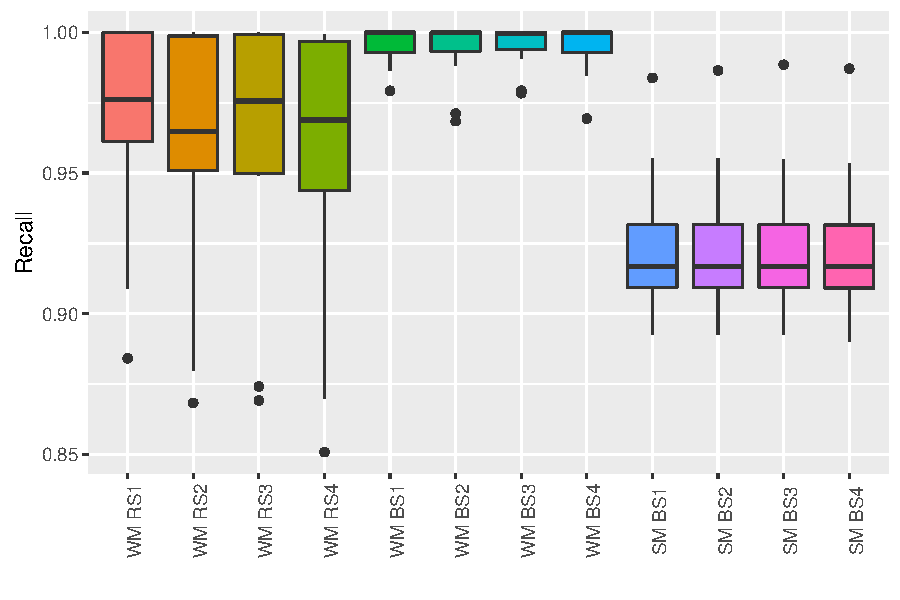
\includegraphics[width=90mm]{mutants-equiv-recall}
	\caption{Non-equivalent mutant classification recall}
	\label{fig:assessment:mutantsequivrecall}
\end{figure}

To answer RQ2, we compute the non-equi\-va\-lent mutant classification recall of the BS/RS algorithms (in Figure \ref{fig:assessment:mutantsequivrecall}), \ie the percentage of non-equi\-va\-lent mutants detected by the BS/RS amongst the selected mutants. By construction, the ALE algorithm has a recall of 100\%, it is therefore not shown here. It is also noted that the precision is 100\% since all the non-equivalent mutants detected are indeed killable, by construction of our mutant set. 

All our simulations obtain a recall higher than 85\%, with a clear advantage for biased simulations which  never achieve worse than  95\% for the weak mutation scenario.  As for time, deviation in the recall is smaller for biased simulations thus making the approach more predictable in addition of being more reliable. We also observe that the random simulations are more sensitive to the number of runs: we need more of them to discover discrepancies by luck. This effect cannot be observed for biased simulations. A possible explanation is that the number of runs required to cover infected states with traces is lower than the number we provided.  

For strong mutation, the BS approach's recall decreases to around 92\% ($\overline{recall}=92$\%, $\sigma=3$\%): amongst the 5113  non-equi\-va\-lent mutant non-detections (over a total of 64529 non-equi\-va\-lent mutant evaluations), 1905 (37\%) were TAD mutants, 1755 (34\%) were WIS mutants, 545 (11\%) were TDE mutants, and 459 (9\%) were 2nd-order TAD mutants (\textit{i.e.}, TAD-TAD mutants); the rest of non-equi\-va\-lent mutants not detected is distributed amongst different operators with less than 2\% for each. This decrease may be due to the difficulty to find a path to the initial state: for strong mutation, the BS trace selection algorithm will consider traces starting from, and ending in, the initial state. This means that mutations creating (TAD) or modifying (TDE) a back-level transition will not be detected using SM BS. Concerning WIS mutants, we believe that, as the WIS operator only changes the initial state of the TS, the set of infected states ($S_{infect}$) is empty, which is equivalent in our implementation of SM BS to considering all the states infected.

\paragraph{Worst case scenario:}
%--------------------------------

\begin{figure}[t]
	\centering
	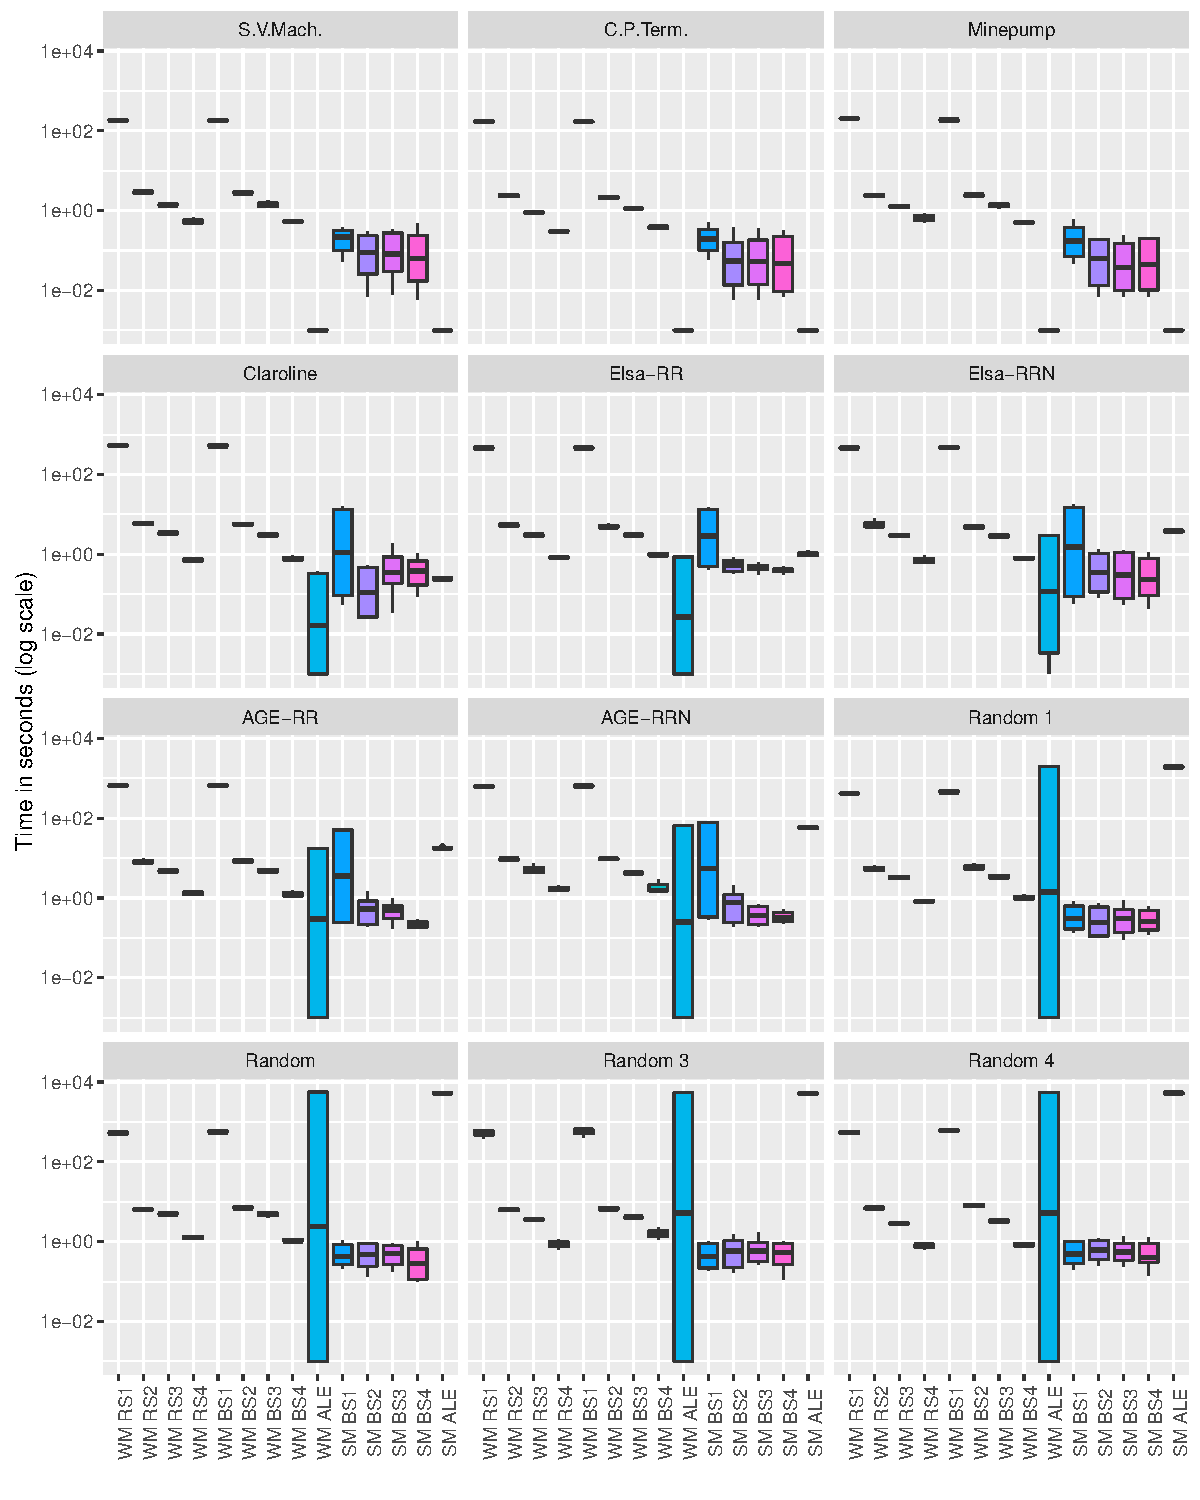
\includegraphics[width=0.98\textwidth]{mutants-equiv-worst}
	\caption{Worst execution time of the equivalent mutant detection using the model itself as mutant}
	\label{fig:assessment:mutantsequivworst}
\end{figure}

Figure \ref{fig:assessment:mutantsequivworst} presents a compact view of the worst execution time of the different algorithms (RQ3). We grouped the different results by the kind of model: embedded system, web-application, or randomly generated model. As expected, the RS/BS execution time is directly correlated to the $\delta$ and $\epsilon$ values: a lower number of traces selected and executed ($N$) takes less time. Overall, the time of the ALE executions grows with the size of the model, reaching 5660 seconds (more than one and a half hour) for the worst WM ALE execution time on the Random~2 model.

%------------------------------
\subsection{Threats to validity}
%------------------------------

\paragraph{Construct validity:}
%-----------------------------

The RS/BS $\delta$ and $\epsilon$ values have been arbitrarily chosen. The first values (RS1/BS1: $\delta=1e-10$, $\epsilon=0.01$) are the same as in H\'erault \etal~\cite{Herault2004}. As the number of traces selected and executed $N$ equals to $\frac{8\log(2/\delta)}{\epsilon^2}$, we chose to run the algorithm with 3 higher parameters values in order to reduce $N$. We cannot guarantee that our parameter values are relevant for any model. They will rather depend on the model size, the desired approximation ($\epsilon$) and confidence ($\delta$), and the time budget allowed for the equivalence analysis.

To the best of our knowledge, the HKC library \cite{hkc} was the only publicly available tool able to perform ALE checking on non-deterministic TSs. We cannot guarantee that there are no other other tools providing the same features with lower execution time. 
To avoid bias in the random selections in the RS/BS algorithms, we execute each configuration of the different algorithms 3 times.

%\paragraph{External validity:}
%%----------------------------
%
%We cannot guarantee that our results are generalizable to all behavioural models. However, we recall the diversity of the model sources (hand-crafted, reverse-engineered, and randomly generated to match real system state-space) as well as the diversity of the considered systems. Variations in performance of the algorithms also suggest mitigation of this threat.

\paragraph{Conclusion validity:}
%-------------------------------

To confirm our observations on the recall of the RS/BS algorithms, we test the null hypothesis between the outputs of our algorithm (the mutant is equivalent/non-equivalent) and a random equivalent/non-equivalent assignment using a Wilcoxon rank sum test. The p-value lower than 2.2e-16\footnote{Due to floating point precision, value $2.2e-16$ corresponds to the smallest possible p-value computable with R.} discredits the null hypothesis showing that the equivalent/non-equivalent detection recall is significant.

\begin{table}
	\centering
	\caption{P-values of the Wilcoxon rank sum test between the WM RS/BS execution times and the WM ALE execution times.}
	\label{tab:assessment:mutantsequivwmpvalues}
	\begin{small} 
\begin{tabular}{lcccc}
%\label{table:WM-pval}
\hline 
\textbf{Model} & \textbf{ WM RS1 } & \textbf{ WM RS2 } & \textbf{ WM RS3 } & \textbf{ WM RS4 } \\ 
\hline 
S.V.Mach.   & $\le 2.2e-16$ & $\le 2.2e-16$ & $\le 2.2e-16$ & $\le 2.2e-16$ \\ 
C.P.Term.   & $\le 2.2e-16$ & $\le 2.2e-16$ & $\le 2.2e-16$ & $\le 2.2e-16$ \\ 
Minepump    & $\le 2.2e-16$ & $\le 2.2e-16$ & $\le 2.2e-16$ & $\le 2.2e-16$ \\ 
Claroline   & $\le 2.2e-16$ & $\le 2.2e-16$ & $\le 2.2e-16$ & $\le 2.2e-16$ \\
Elsa-RR     & $\le 2.2e-16$ & $\le 2.2e-16$ & $\le 2.2e-16$ & $\le 2.2e-16$ \\
Elsa-RRN   & $\le 2.2e-16$ & $\le 2.2e-16$ & $\le 2.2e-16$ & $\le 2.2e-16$ \\
AGE-RR   & $2.866e-03$ & $9.676e-03$ & $2.021e-02$ & $\mathbf{3.249e-01}$ \\
AGE-RRN   & $\mathbf{8.143e-02}$ & $8.379e-04$ & $6.981e-04$ & $2.162e-02$ \\
Random 1   & $\le 2.2e-16$ & $\le 2.2e-16$ & $\le 2.2e-16$ & $\le 2.2e-16$ \\
Random 2   & $\le 2.2e-16$ & $\le 2.2e-16$ & $\le 2.2e-16$ & $\le 2.2e-16$ \\
Random 3   & $\le 2.2e-16$ & $\le 2.2e-16$ & $\le 2.2e-16$ & $\le 2.2e-16$ \\
Random 4   & $\le 2.2e-16$ & $\le 2.2e-16$ & $\le 2.2e-16$ & $\le 2.2e-16$ \\
\hline 
\end{tabular} 
\end{small}

\vspace{1em}

\begin{small} 
\begin{tabular}{lcccc}
%\label{table:WM-pval}
\hline 
\textbf{Model} & \textbf{ WM BS1 } & \textbf{ WM BS2 } & \textbf{ WM BS3 } & \textbf{ WM BS4 } \\ 
\hline 
S.V.Mach.   & $\le 2.2e-16$ & $\le 2.2e-16$ & $\le 2.2e-16$ & $\le 2.2e-16$\\ 
C.P.Term.   & $\le 2.2e-16$ & $\le 2.2e-16$ & $\le 2.2e-16$ & $\le 2.2e-16$\\ 
Minepump    & $\le 2.2e-16$ & $\le 2.2e-16$ & $\le 2.2e-16$ & $\le 2.2e-16$\\ 
Claroline   & $\le 2.2e-16$ & $\le 2.2e-16$ & $\le 2.2e-16$ & $\le 2.2e-16$\\ 
Elsa-RR     & $\le 2.2e-16$ & $\le 2.2e-16$ & $\le 2.2e-16$ & $\le 2.2e-16$\\ 
Elsa-RRN    & $\le 2.2e-16$ & $\le 2.2e-16$ & $\le 2.2e-16$ & $\le 2.2e-16$\\ 
AGE-RR      & $9.107e-03$ & $4.744e-02$ & $\mathbf{6.405e-02}$ & $\mathbf{1.382e-01}$\\ 
AGE-RRN     & $\mathbf{5.991e-01}$ & $\mathbf{7.076e-01}$ & $\mathbf{5.674e-01}$ & $\mathbf{5.168e-01}$\\ 
Random 1    & $\le 2.2e-16$ & $\le 2.2e-16$ & $\le 2.2e-16$ & $\le 2.2e-16$\\ 
Random 2    & $\le 2.2e-16$ & $\le 2.2e-16$ & $\le 2.2e-16$ & $\le 2.2e-16$\\ 
Random 3    & $\le 2.2e-16$ & $\le 2.2e-16$ & $\le 2.2e-16$ & $\le 2.2e-16$\\ 
Random 4    & $\le 2.2e-16$ & $\le 2.2e-16$ & $\le 2.2e-16$ & $\le 2.2e-16$\\ 
\hline 
\end{tabular} 
\end{small}

\end{table}

To confirm the statistical difference between the execution times of the RS/BS and ALE algorithms, we test the null hypothesis between RS/BS execution time and ALE execution time for weak and strong mutation for each of our input models using a Wilcoxon rank sum test. For weak mutation, the results of this statistical test are shown in Table \ref{tab:assessment:mutantsequivwmpvalues}: for every model except \textit{AGE-RR}/\textit{AGE-RRN} models, the p-value is lower than 2.2e-16, discrediting the null hypothesis and showing a significant difference in the execution times. The execution times of \textit{AGE-RR}/\textit{AGE-RRN} model are only significant for RS1 to RS3, BS1, and BS3 (for \textit{AGE-RR}); and RS2 to RS4 (for \textit{AGE-RRN}). For strong mutation, all the p-values were lower than 2.2e-16, showing a significant difference in execution time between the BS algorithm and the ALE algorithm in a strong mutation scenario.


%------------------------------
\subsection{Lessons learned}
%------------------------------

From our experiment we draw the following lessons: 
\begin{inparaenum}
\item regarding weak mutation and independently of the size or nature of the models, the ALE approach provides faster and exact answers. This indicates that state-of-the-art language equivalence algorithms can be used successfully for such a task.
\item Regarding strong mutation, biased random simulations are of interest for the web and the random models, and gains increase with the size (from one to three orders of magnitude).  Recalls of 90\% and above allow to use such simulations as reasonably reliable fast filters to discard non-equivalent mutants, leaving to ALE algorithms ``difficult" cases so as to accelerate the analysis of large mutants bases.
\item Biased simulations are more predictable in terms of execution time and recall. Additionally, drastically increasing the number of runs does not affect their performance as opposed to random simulations.    
\item The configuration of the ALE algorithm (forward/backward processing, or breadth-first or depth-first exploration) has very little influence on the total execution time (regarding equivalent mutant detection). This may be explained by the fact that mutations occur randomly and therefore do not privilege any graph traversal strategy.  
\end{inparaenum}


%%%%%%%%%%%%%%%%%%%%%%%%%%%%%%%%%%%%
\section{Wrap up}
%%%%%%%%%%%%%%%%%%%%%%%%%%%%%%%%%%%%

This chapter presents the empirical assessment and their results validating the the selection criteria and mutation analysis described in Chapters \ref{chap:coverage} and \ref{chap:mutation}. Future work include generalisation of the results by using all the case studies from Chapter \ref{chap:casestudies} for each assessment and comparison of the different test suite selection criteria using mutation analysis. 








